\chapter{Resultados}
\label{cap:resultados}

\section{Caracterização da Base e Análise Exploratória}

Após a aplicação dos procedimentos de preparação descritos na
\cref{cap:metodologia}, a base reuniu 401\,087 registros válidos. A
\cref{tab:base-dados-resultados} resume as quantidades observadas nas etapas
iniciais. O conjunto agregado das quatro granularidades totalizou 642\,938
linhas; esse total corresponde à representação da mesma série em diferentes
resoluções temporais e, portanto, não deve ser interpretado como quantidade
de observações independentes.

\begin{table}[H]
  \centering
  \caption{Síntese quantitativa da base de dados.}
  \label{tab:base-dados-resultados}
  \begin{tabular}{lr}
    \toprule
    Descrição & Quantidade \\
    \midrule
    Registros brutos & 410\,451 \\
    Registros sem valor de PCA removidos & 76 \\
    Registros após os filtros de qualidade & 401\,087 \\
    Leituras com PCA igual a zero na base bruta & 9\,607 (2,3\%) \\
    Linhas no conjunto agregado das quatro granularidades & 642\,938 \\
    \bottomrule
  \end{tabular}
  \source{Elaborado pelo autor.}
\end{table}

A distribuição das amostras de E1 entre as partições temporais variou de
acordo com a granularidade. A \cref{tab:splits-resultados} apresenta as
quantidades utilizadas no treinamento, na validação e calibração e no teste.

\begin{table}[H]
  \centering
  \caption{Quantidade de amostras por granularidade e partição temporal do inversor E1.}
  \label{tab:splits-resultados}
  \resizebox{\textwidth}{!}{%
  \begin{tabular}{lrrr}
    \toprule
    Granularidade & Treinamento (2021--2024H1) & Validação e calibração (2024H2) & Teste (2025) \\
    \midrule
    5 min  & 156\,440 & 22\,533 & 44\,911 \\
    10 min & 79\,065  & 11\,366 & 22\,637 \\
    1 h    & 14\,133  & 2\,033  & 4\,042 \\
    1 d    & 1\,250   & 182     & 354 \\
    \bottomrule
  \end{tabular}}
  \source{Elaborado pelo autor.}
\end{table}

As séries dos três inversores apresentaram lacunas de telemetria. A ausência
correspondeu a 13,68\% dos períodos diurnos esperados no E1, 13,45\% no E2 e
13,43\% no E3. A maior lacuna contínua observada foi de 12~h. O maior
percentual anual de ausência ocorreu no E1 em 2022, quando 17,1\% dos
períodos esperados não possuíam registro. Esses valores caracterizam a
integridade das séries utilizadas e contextualizam o ensaio com lacunas
artificiais apresentado na \cref{sec:ensaio-embarcado}.

O perfil horário da potência ativa CA apresentou valores mais baixos no
início e no fim do período diurno e valores máximos próximos ao meio-dia,
conforme a \cref{fig:pca-horaria}. Esse comportamento corresponde ao perfil
diário observado para a geração fotovoltaica.

\begin{figure}[H]
  \centering
  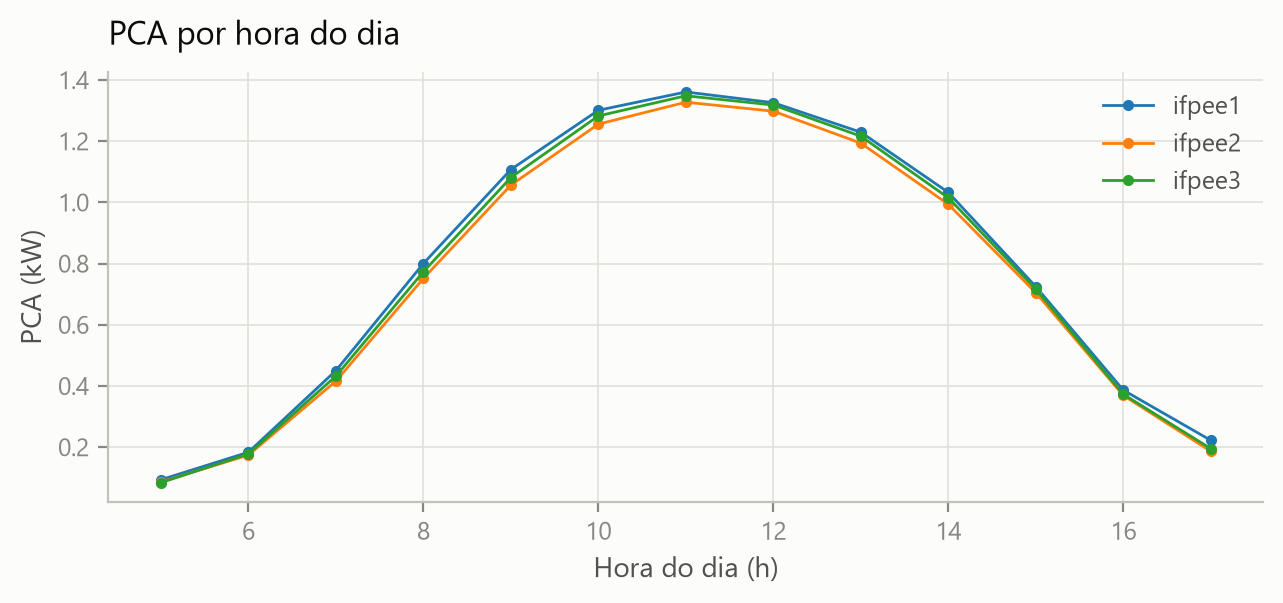
\includegraphics[width=0.92\textwidth]{figuras/pca_por_hora_do_dia.png}
  \caption{Perfil horário da potência ativa CA dos inversores ao longo do período diurno.}
  \label{fig:pca-horaria}
  \source{Elaborado pelo autor.}
\end{figure}

A razão mensal entre PCA e irradiância transposta para o plano dos módulos
($\mathrm{PCA}/\mathrm{ghit}$) apresentou valores inferiores a partir de 2024
em relação à média de 2021 a 2023, como mostra a \cref{fig:produtividade}.
Essa razão foi utilizada apenas como indicador descritivo da evolução do
desempenho do sistema; não integrou o conjunto de características de entrada
nem o treinamento dos modelos.

\begin{figure}[H]
  \centering
  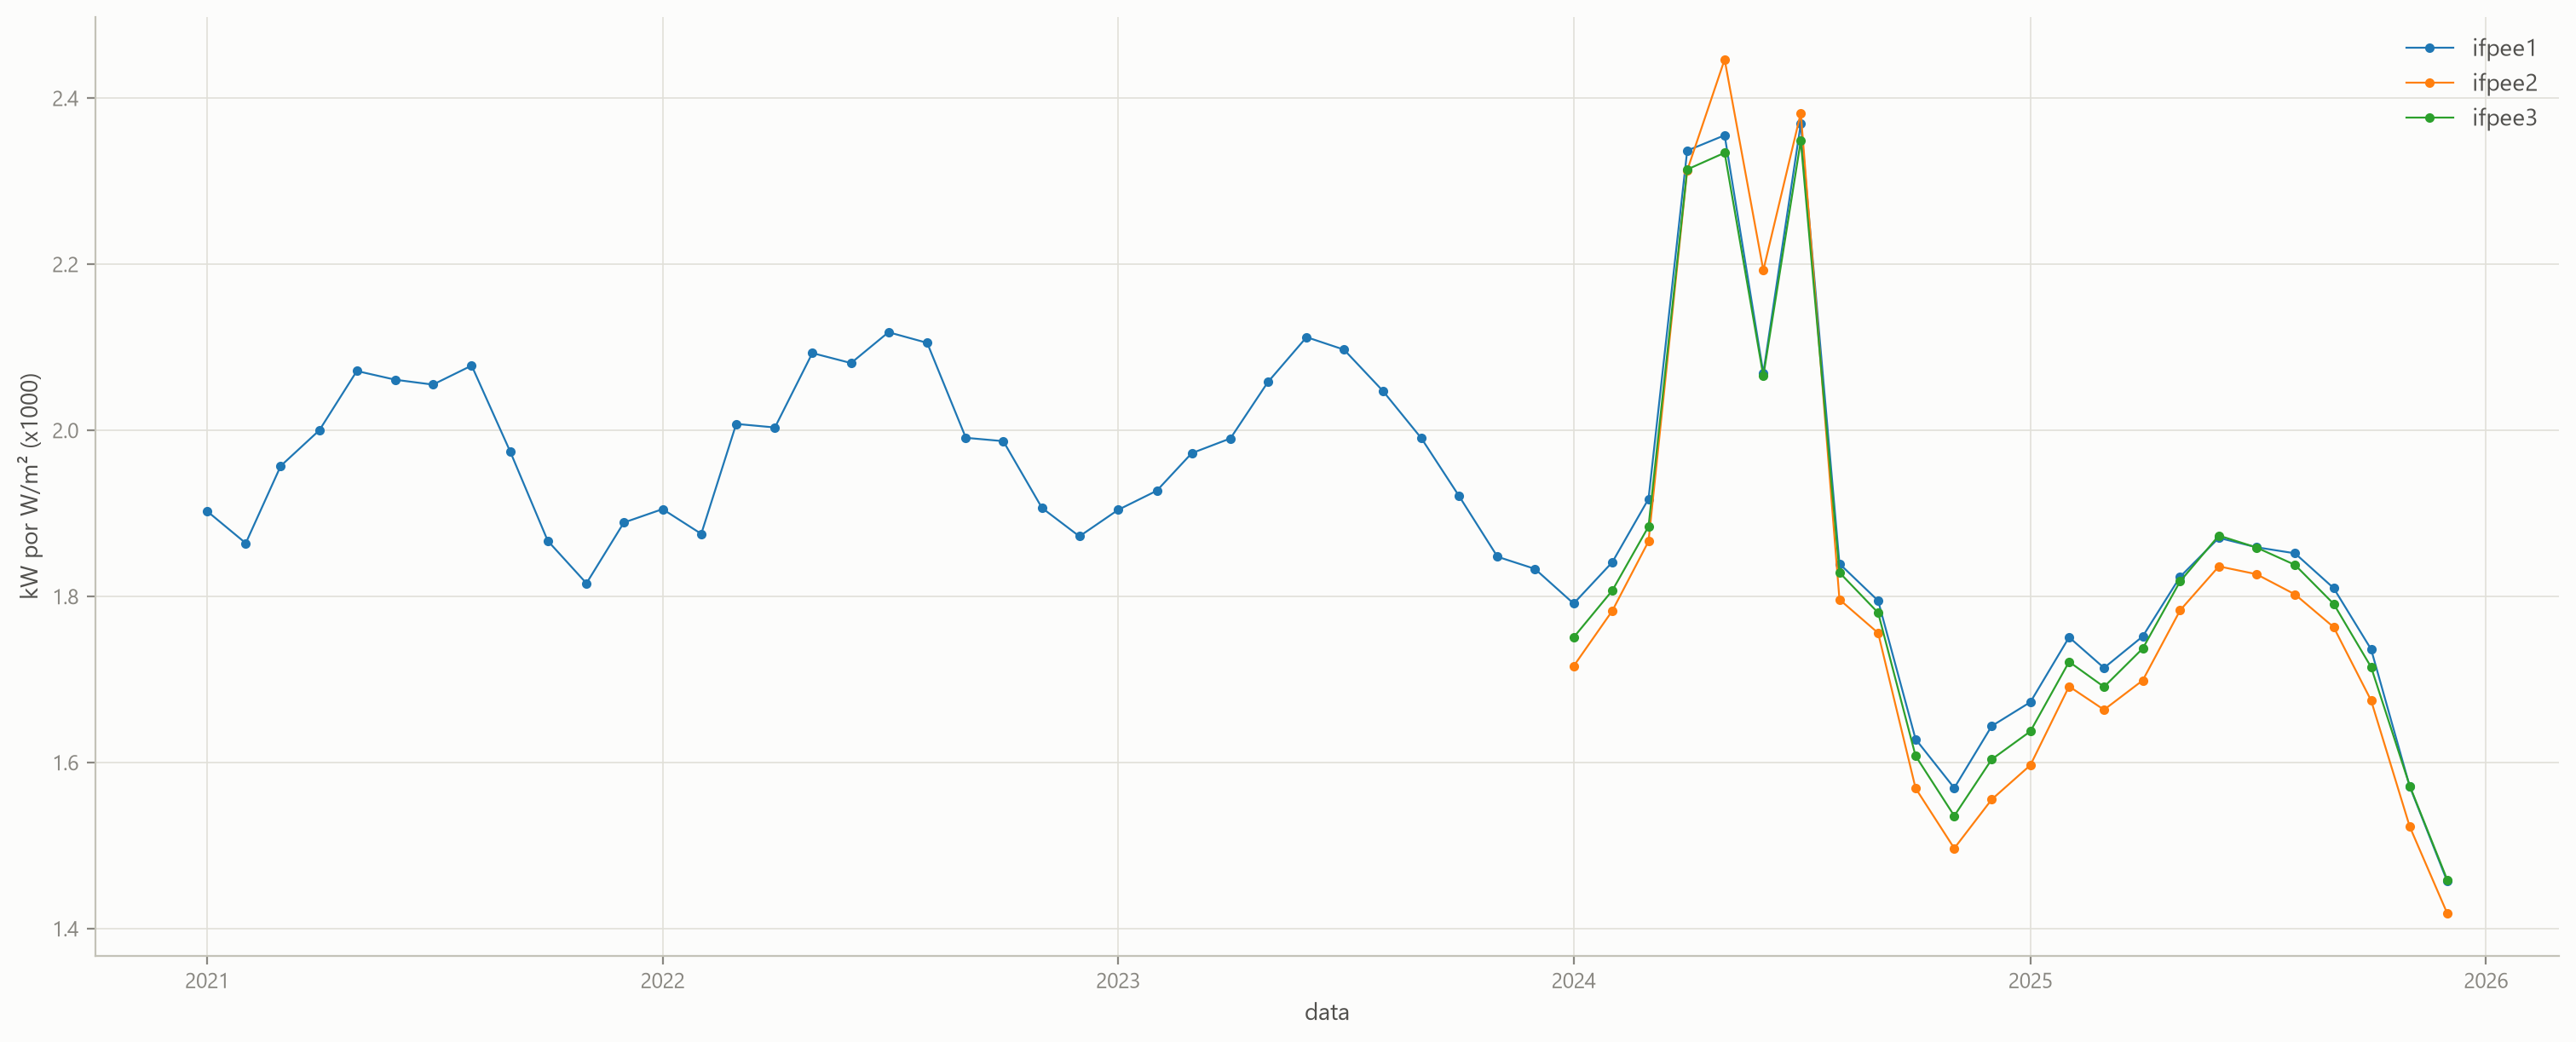
\includegraphics[width=0.92\textwidth]{figuras/produtividade.png}
  \caption{Evolução mensal da razão entre potência ativa CA e irradiância transposta para o plano dos módulos.}
  \label{fig:produtividade}
  \source{Elaborado pelo autor.}
\end{figure}

A \cref{fig:matriz-correlacao} apresenta a matriz de correlação das variáveis
examinadas na análise exploratória, incluindo as grandezas meteorológicas e
as estimativas alternativas de temperatura de módulo disponíveis na base.
A inspeção foi utilizada na caracterização das relações entre as variáveis e
na análise das três características adotadas pelos modelos.

\begin{figure}[H]
  \centering
  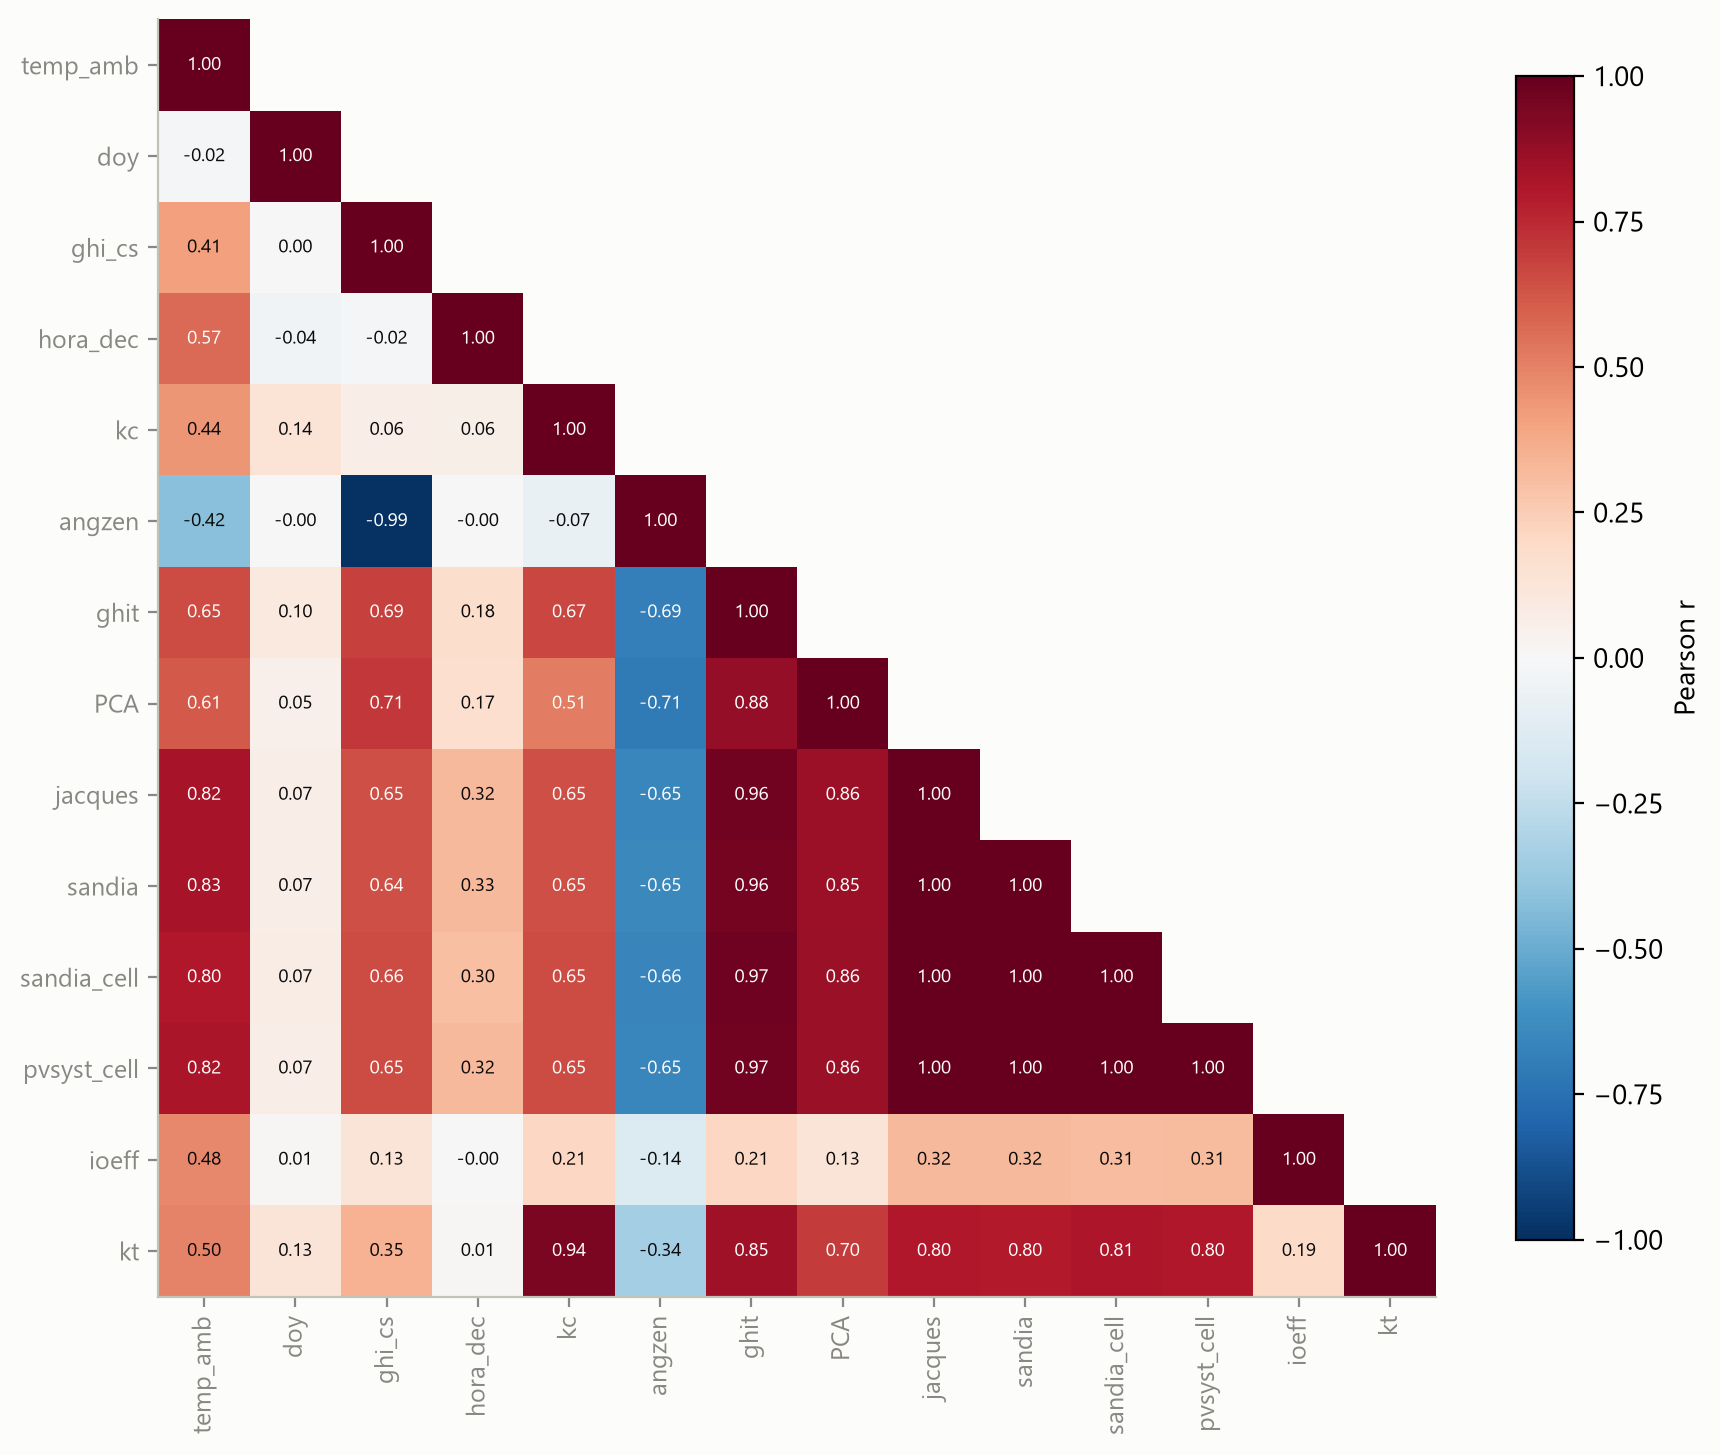
\includegraphics[width=0.88\textwidth]{figuras/matriz_correlacao_variaveis.png}
  \caption{Matriz de correlação das variáveis examinadas na análise exploratória.}
  \label{fig:matriz-correlacao}
  \source{Elaborado pelo autor.}
\end{figure}

A inspeção da PACF e da IACF da série horária de PCA não indicou dependência
temporal que justificasse a inclusão de variáveis defasadas. Esse resultado
é compatível com a formulação contemporânea adotada, na qual as características
do intervalo são associadas à potência do mesmo intervalo.

A distribuição da potência foi examinada em 5~min, 10~min, 30~min, 1~h,
6~h e 1~d. A \cref{fig:pca-distribuicao} reúne as distribuições observadas.
Em todas as resoluções, houve concentração de valores em potências baixas
e uma cauda que se estendeu até a região de saturação do inversor, próxima
de 2~kW. A assimetria também pode ser observada nas distribuições após a
transformação Box--Cox, apresentadas para as quatro granularidades utilizadas
no treinamento na \cref{fig:pca-boxcox}.

\begin{figure}[H]
  \centering
  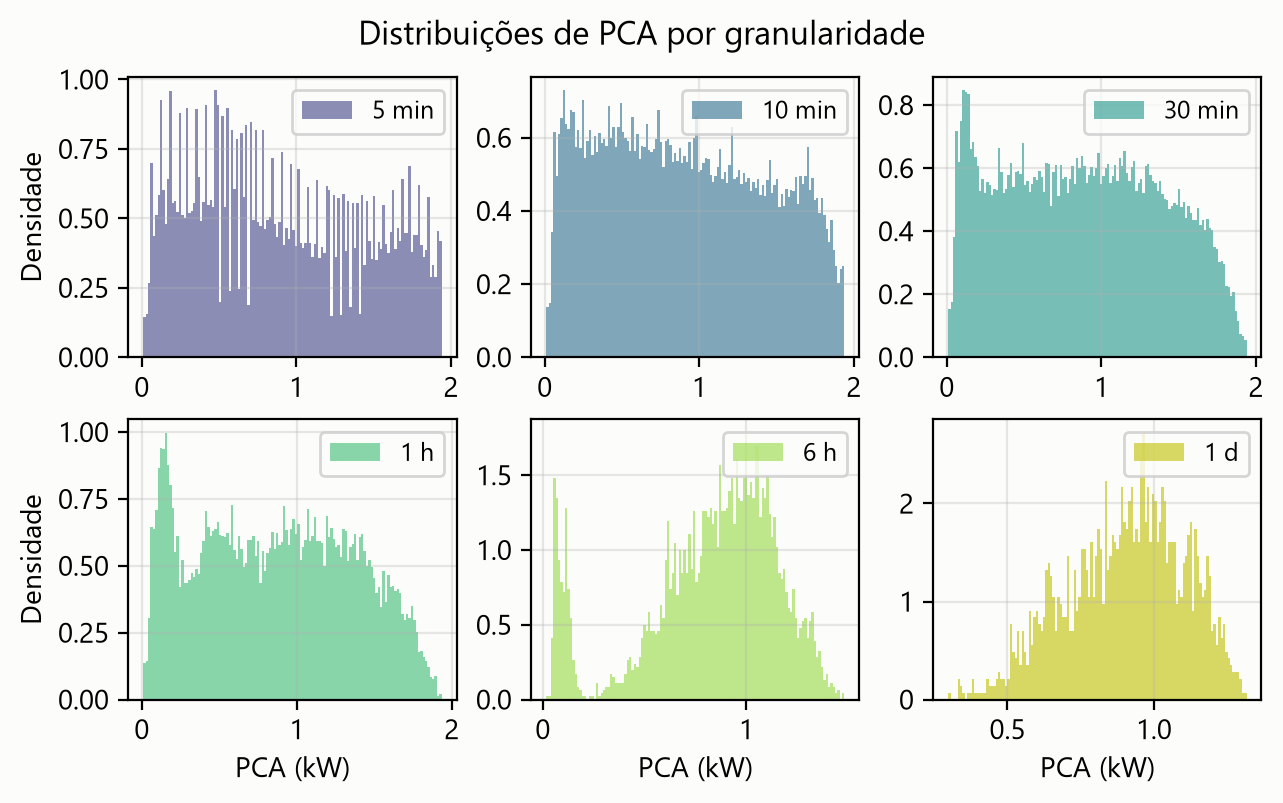
\includegraphics[width=0.92\textwidth]{figuras/pca_distribuicao_granularidades.png}
  \caption{Distribuição da potência ativa CA nas diferentes granularidades examinadas.}
  \label{fig:pca-distribuicao}
  \source{Elaborado pelo autor.}
\end{figure}

\begin{figure}[H]
  \centering
  \begin{minipage}[t]{0.48\textwidth}
    \centering
    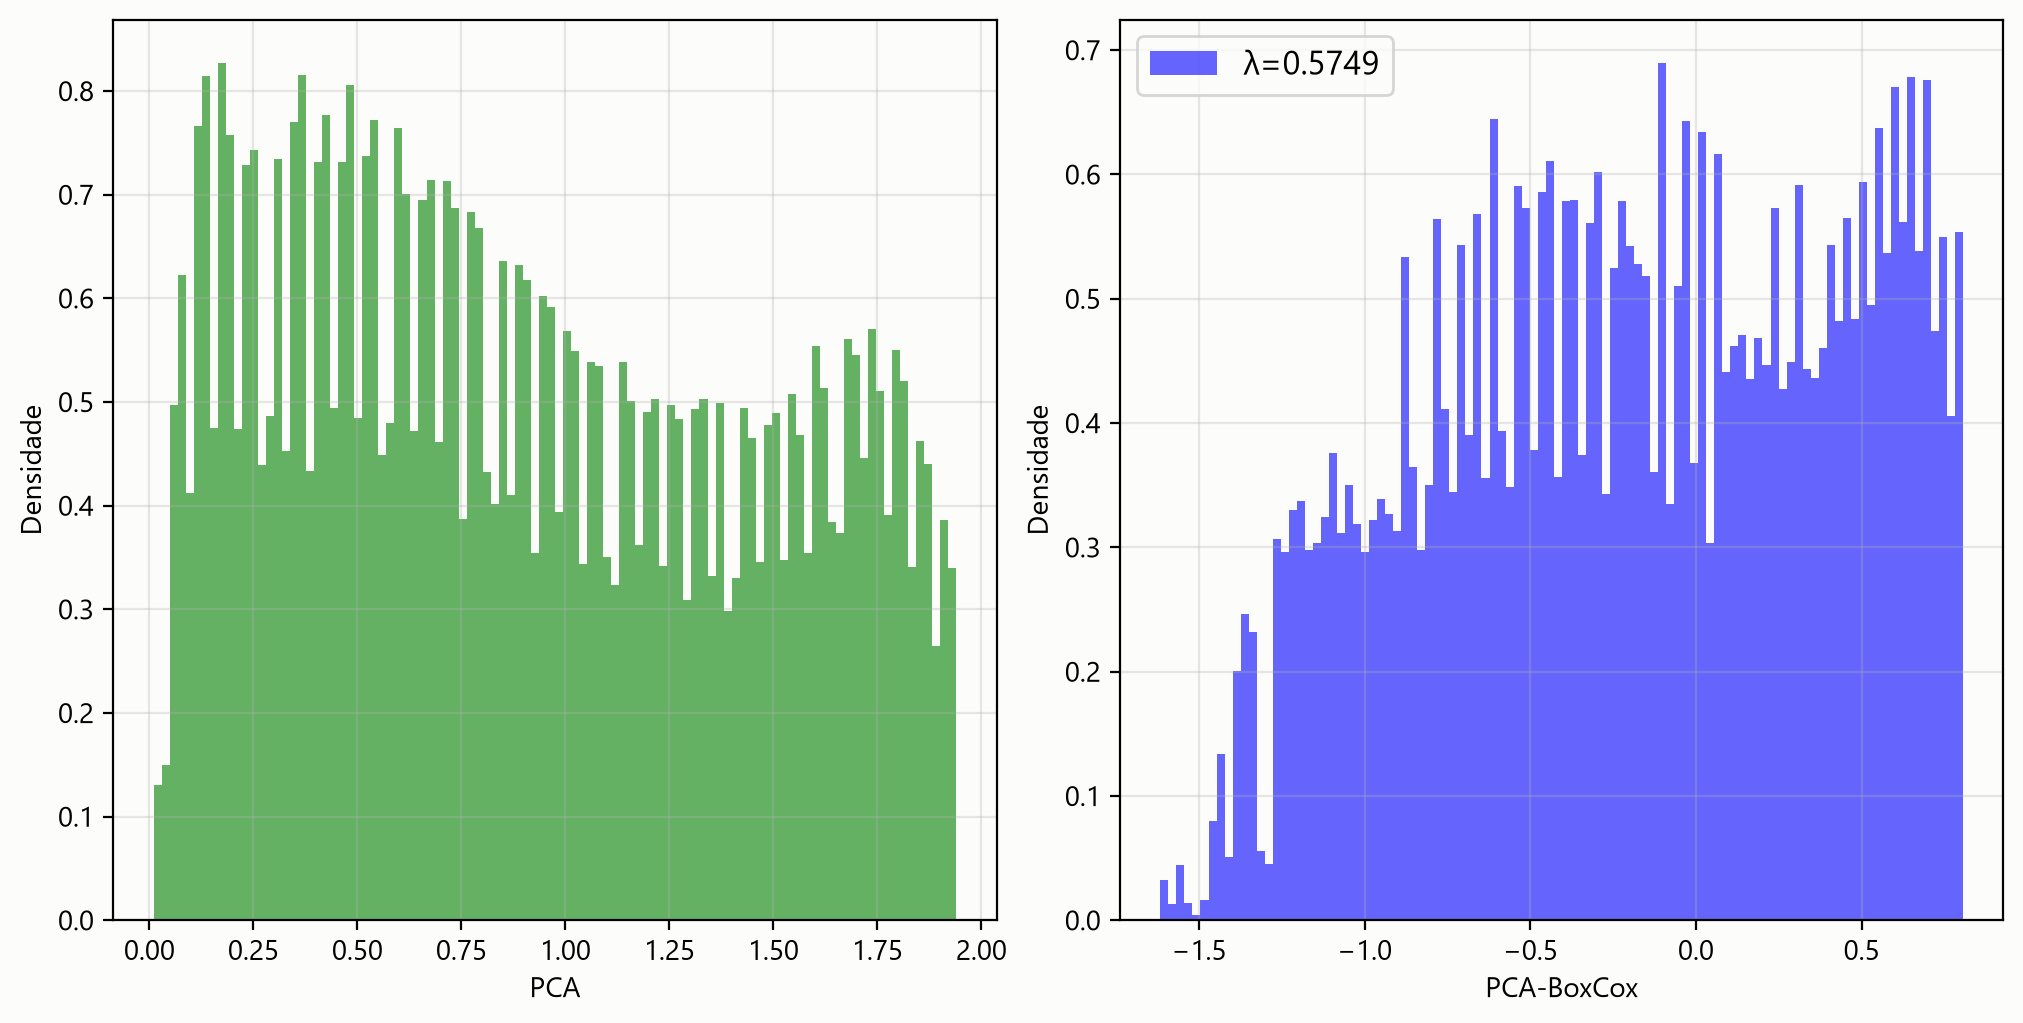
\includegraphics[width=\linewidth]{figuras/pca_boxcox_distribution_5min.png}
    \par\small (a) 5 min
  \end{minipage}\hfill
  \begin{minipage}[t]{0.48\textwidth}
    \centering
    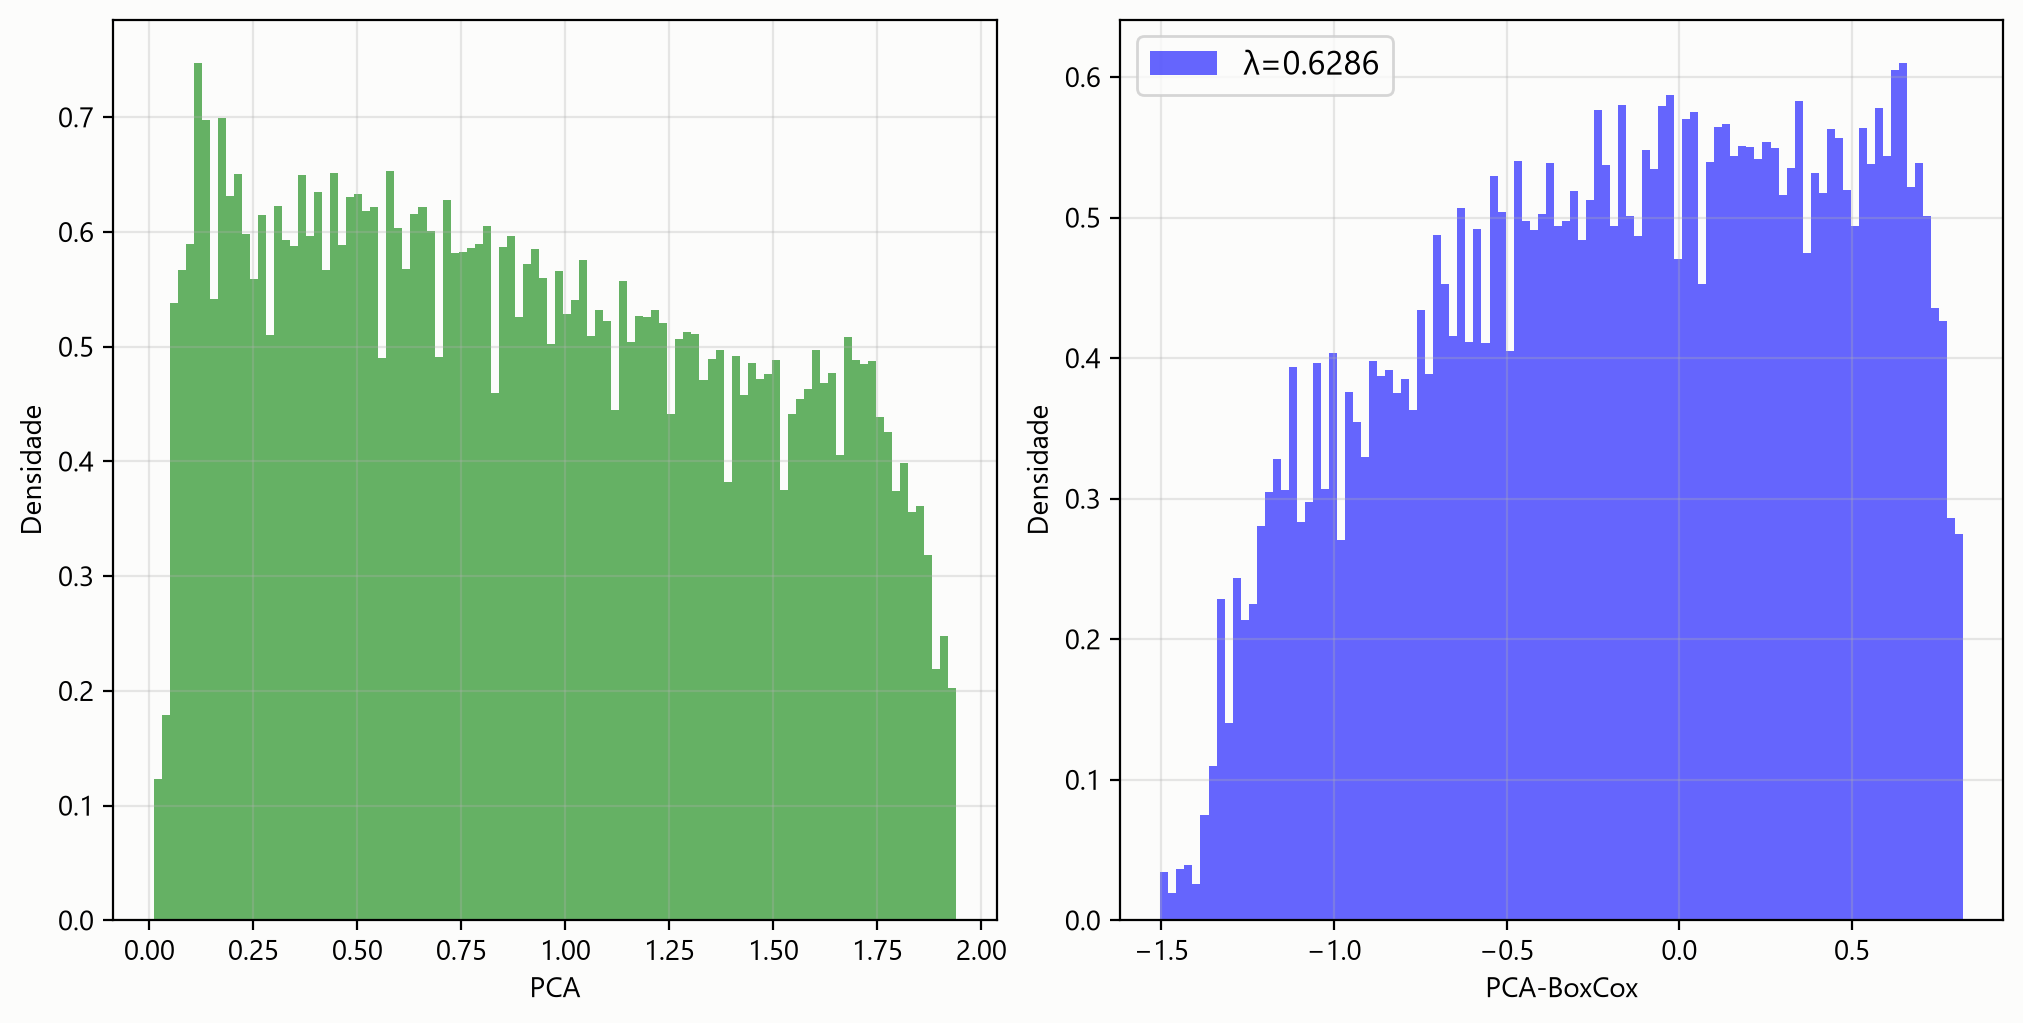
\includegraphics[width=\linewidth]{figuras/pca_boxcox_distribution_10min.png}
    \par\small (b) 10 min
  \end{minipage}
  \vspace{0.5em}
  \begin{minipage}[t]{0.48\textwidth}
    \centering
    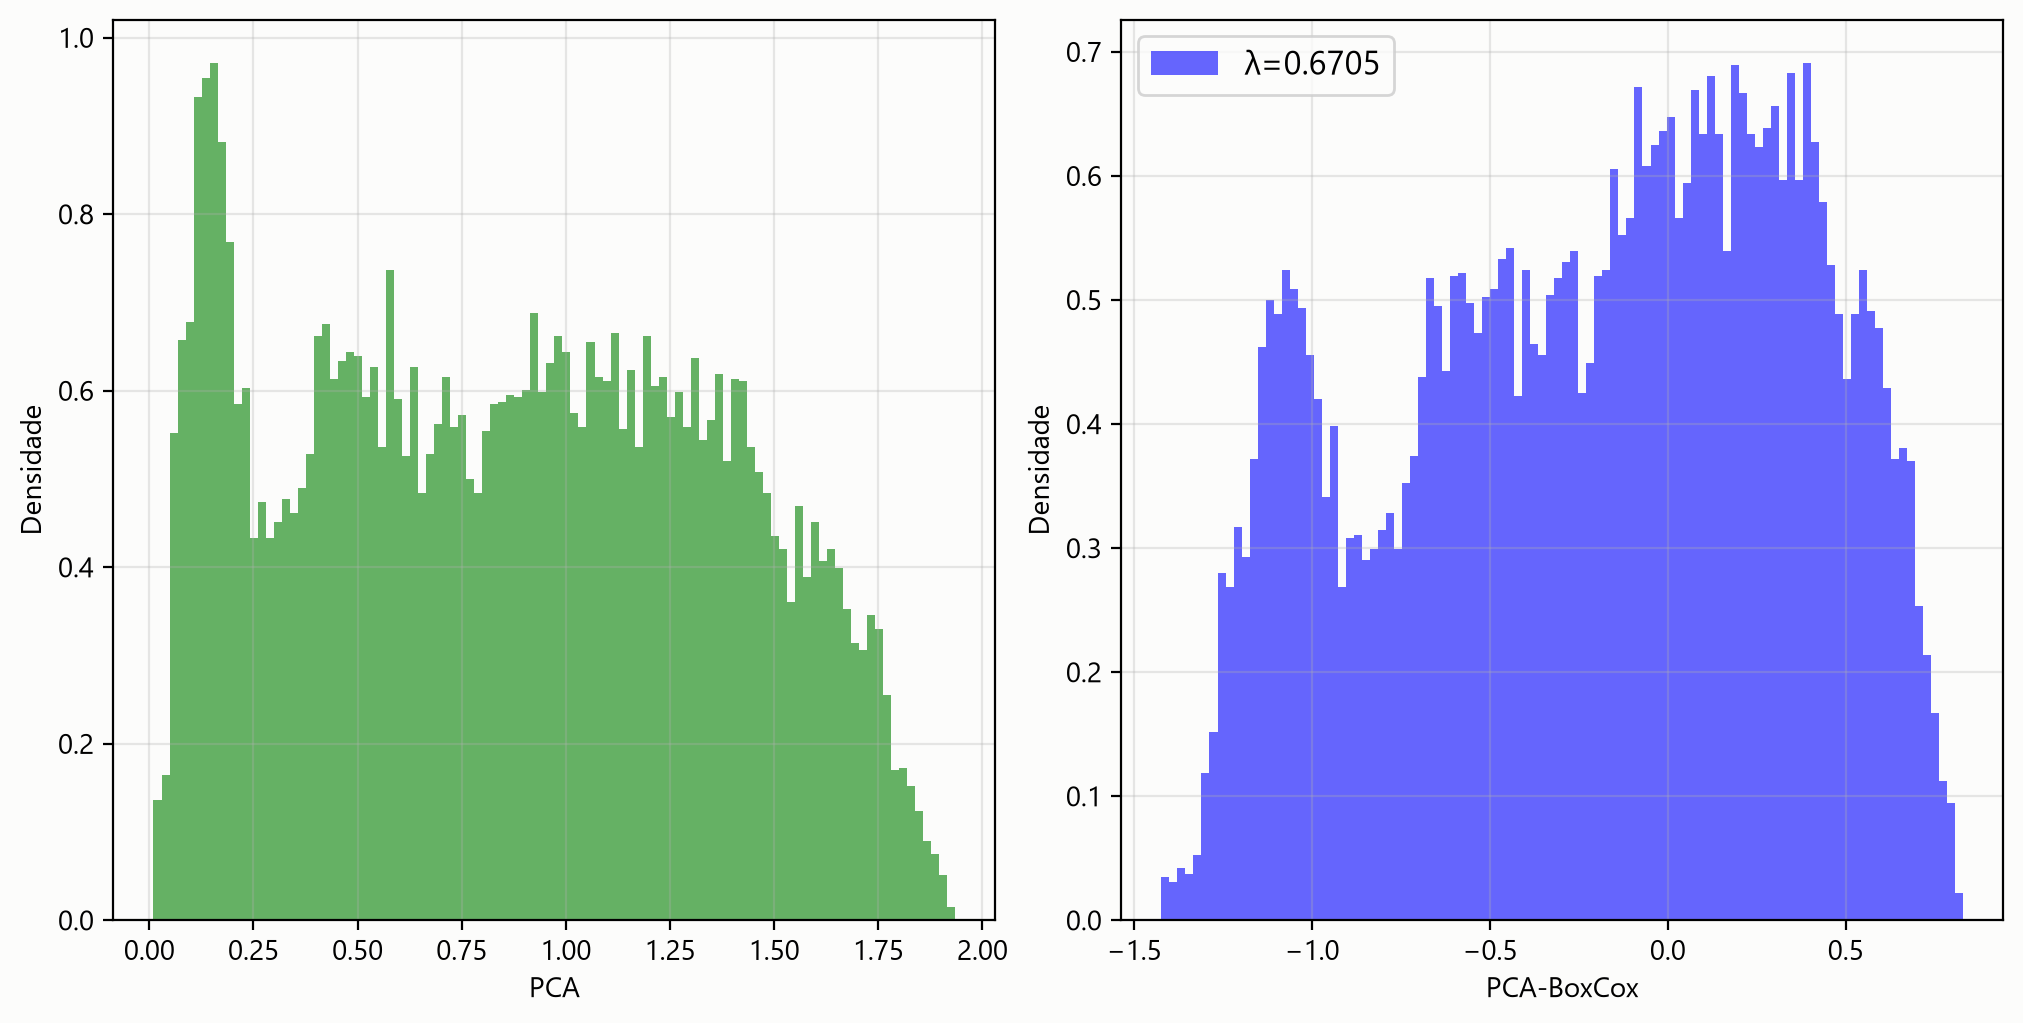
\includegraphics[width=\linewidth]{figuras/pca_boxcox_distribution_1h.png}
    \par\small (c) 1 h
  \end{minipage}\hfill
  \begin{minipage}[t]{0.48\textwidth}
    \centering
    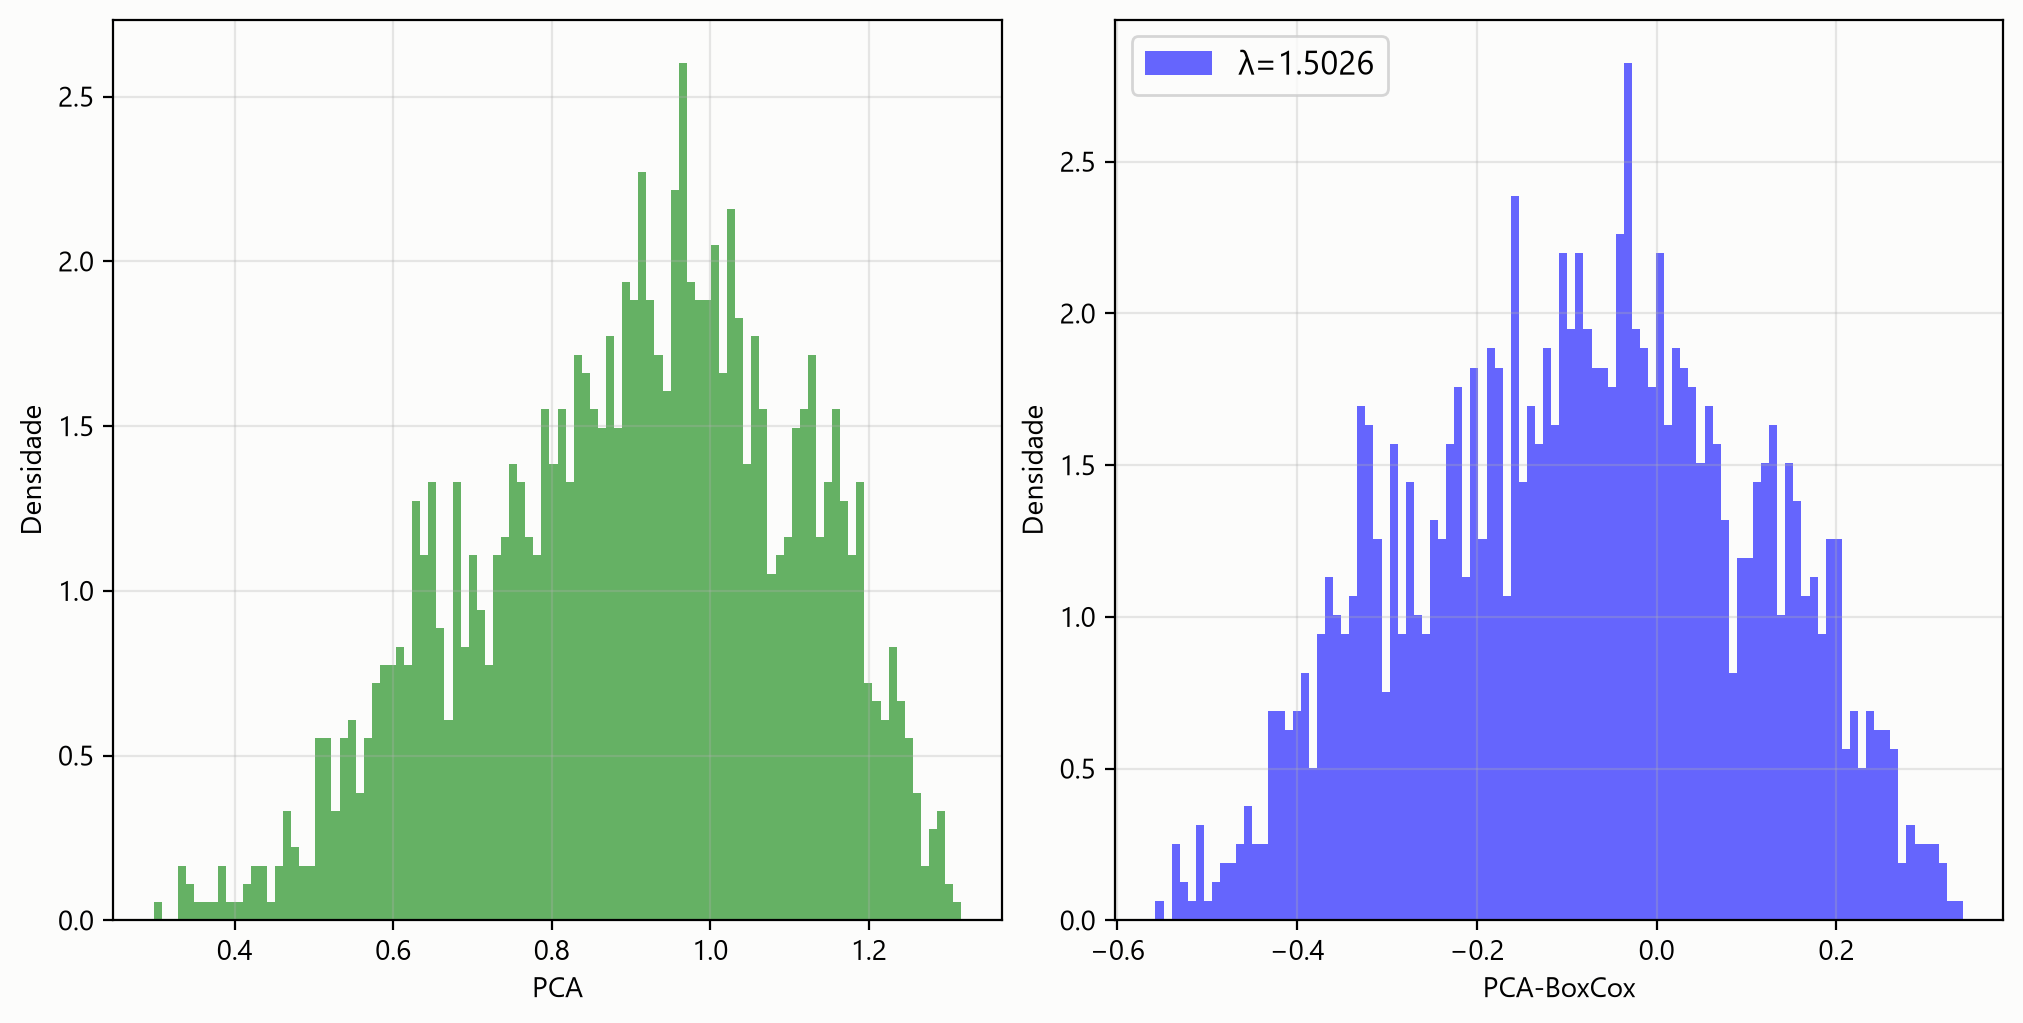
\includegraphics[width=\linewidth]{figuras/pca_boxcox_distribution_1D.png}
    \par\small (d) 1 d
  \end{minipage}
  \caption{Distribuições do alvo após a transformação Box--Cox nas quatro granularidades utilizadas no treinamento dos modelos.}
  \label{fig:pca-boxcox}
  \source{Elaborado pelo autor.}
\end{figure}

\section{Treinamento e Convergência}

A \cref{tab:rf-custo-treinamento} apresenta a quantidade de nós das florestas
selecionadas, os tempos de treinamento e os tempos médios de inferência
medidos no host. O tempo de treinamento variou entre 0,1~s e 0,6~s. O tempo
de inferência por amostra aumentou com a complexidade observada da floresta,
atingindo 216,1~$\mu$s na granularidade diária.

\begin{table}[H]
  \centering
  \caption{Complexidade e tempos medidos para os modelos Random Forest.}
  \label{tab:rf-custo-treinamento}
  \begin{tabular}{lrrr}
    \toprule
    Granularidade & Nós & Treinamento (s) & Inferência ($\mu$s/amostra) \\
    \midrule
    5 min  & 3\,012  & 0,5 & 0,9 \\
    10 min & 7\,585  & 0,6 & 2,4 \\
    1 h    & 34\,578 & 0,3 & 24,9 \\
    1 d    & 11\,140 & 0,1 & 216,1 \\
    \bottomrule
  \end{tabular}
  \source{Elaborado pelo autor.}
\end{table}

Para a biblioteca C de 1~h, o cabeçalho gerado registrou MAE de
0,0666~kW, $R^2=0,9716$ e correção de calibração de $-0,106076$~kW. Esses
valores diferem ligeiramente dos obtidos no notebook para o modelo de
referência (MAE de 0,0664~kW e $R^2=0,9717$). A biblioteca foi gerada a partir
de um arquivo \texttt{joblib} salvo em uma execução ligeiramente anterior,
o que explica a pequena diferença entre os artefatos.

No MLP, o treinamento foi encerrado antes do limite máximo de épocas em
todas as granularidades. A \cref{tab:mlp-treinamento} reúne os valores de
$\lambda$ estimados para a transformação Box--Cox, as correções de calibração,
o número de épocas efetivamente executadas e os tempos medidos. O deslocamento
de $0{,}001$~kW utilizado na transformação do alvo não está incluído na coluna
de correção de calibração, pois corresponde a uma operação distinta.

\begin{table}[H]
  \centering
  \caption{Parâmetros estimados e tempos de treinamento do MLP por granularidade.}
  \label{tab:mlp-treinamento}
  \begin{tabular}{lrrrr}
    \toprule
    Granularidade & $\lambda$ & Correção de calibração (kW) & Épocas executadas & Treinamento (s) \\
    \midrule
    5 min  & 0,5665 & $-0,0387$ & 155 & 264,5 \\
    10 min & 0,6138 & $-0,0758$ & 128 & 95,5 \\
    1 h    & 0,6514 & $-0,0594$ & 87  & 39,5 \\
    1 d    & 1,4133 & $-0,0514$ & 123 & 16,2 \\
    \bottomrule
  \end{tabular}
  \source{Elaborado pelo autor.}
\end{table}

O menor MAE de validação no espaço transformado foi 0,19859 em 5~min,
0,15798 em 10~min, 0,09699 em 1~h e 0,05558 em 1~d. A
\cref{fig:mlp-treino} apresenta a evolução das métricas de treinamento e
validação nas quatro granularidades. Para 1~h, a
\cref{fig:mlp-treino-1h} detalha as curvas de perda, MAE e RMSE.

\begin{figure}[H]
  \centering
  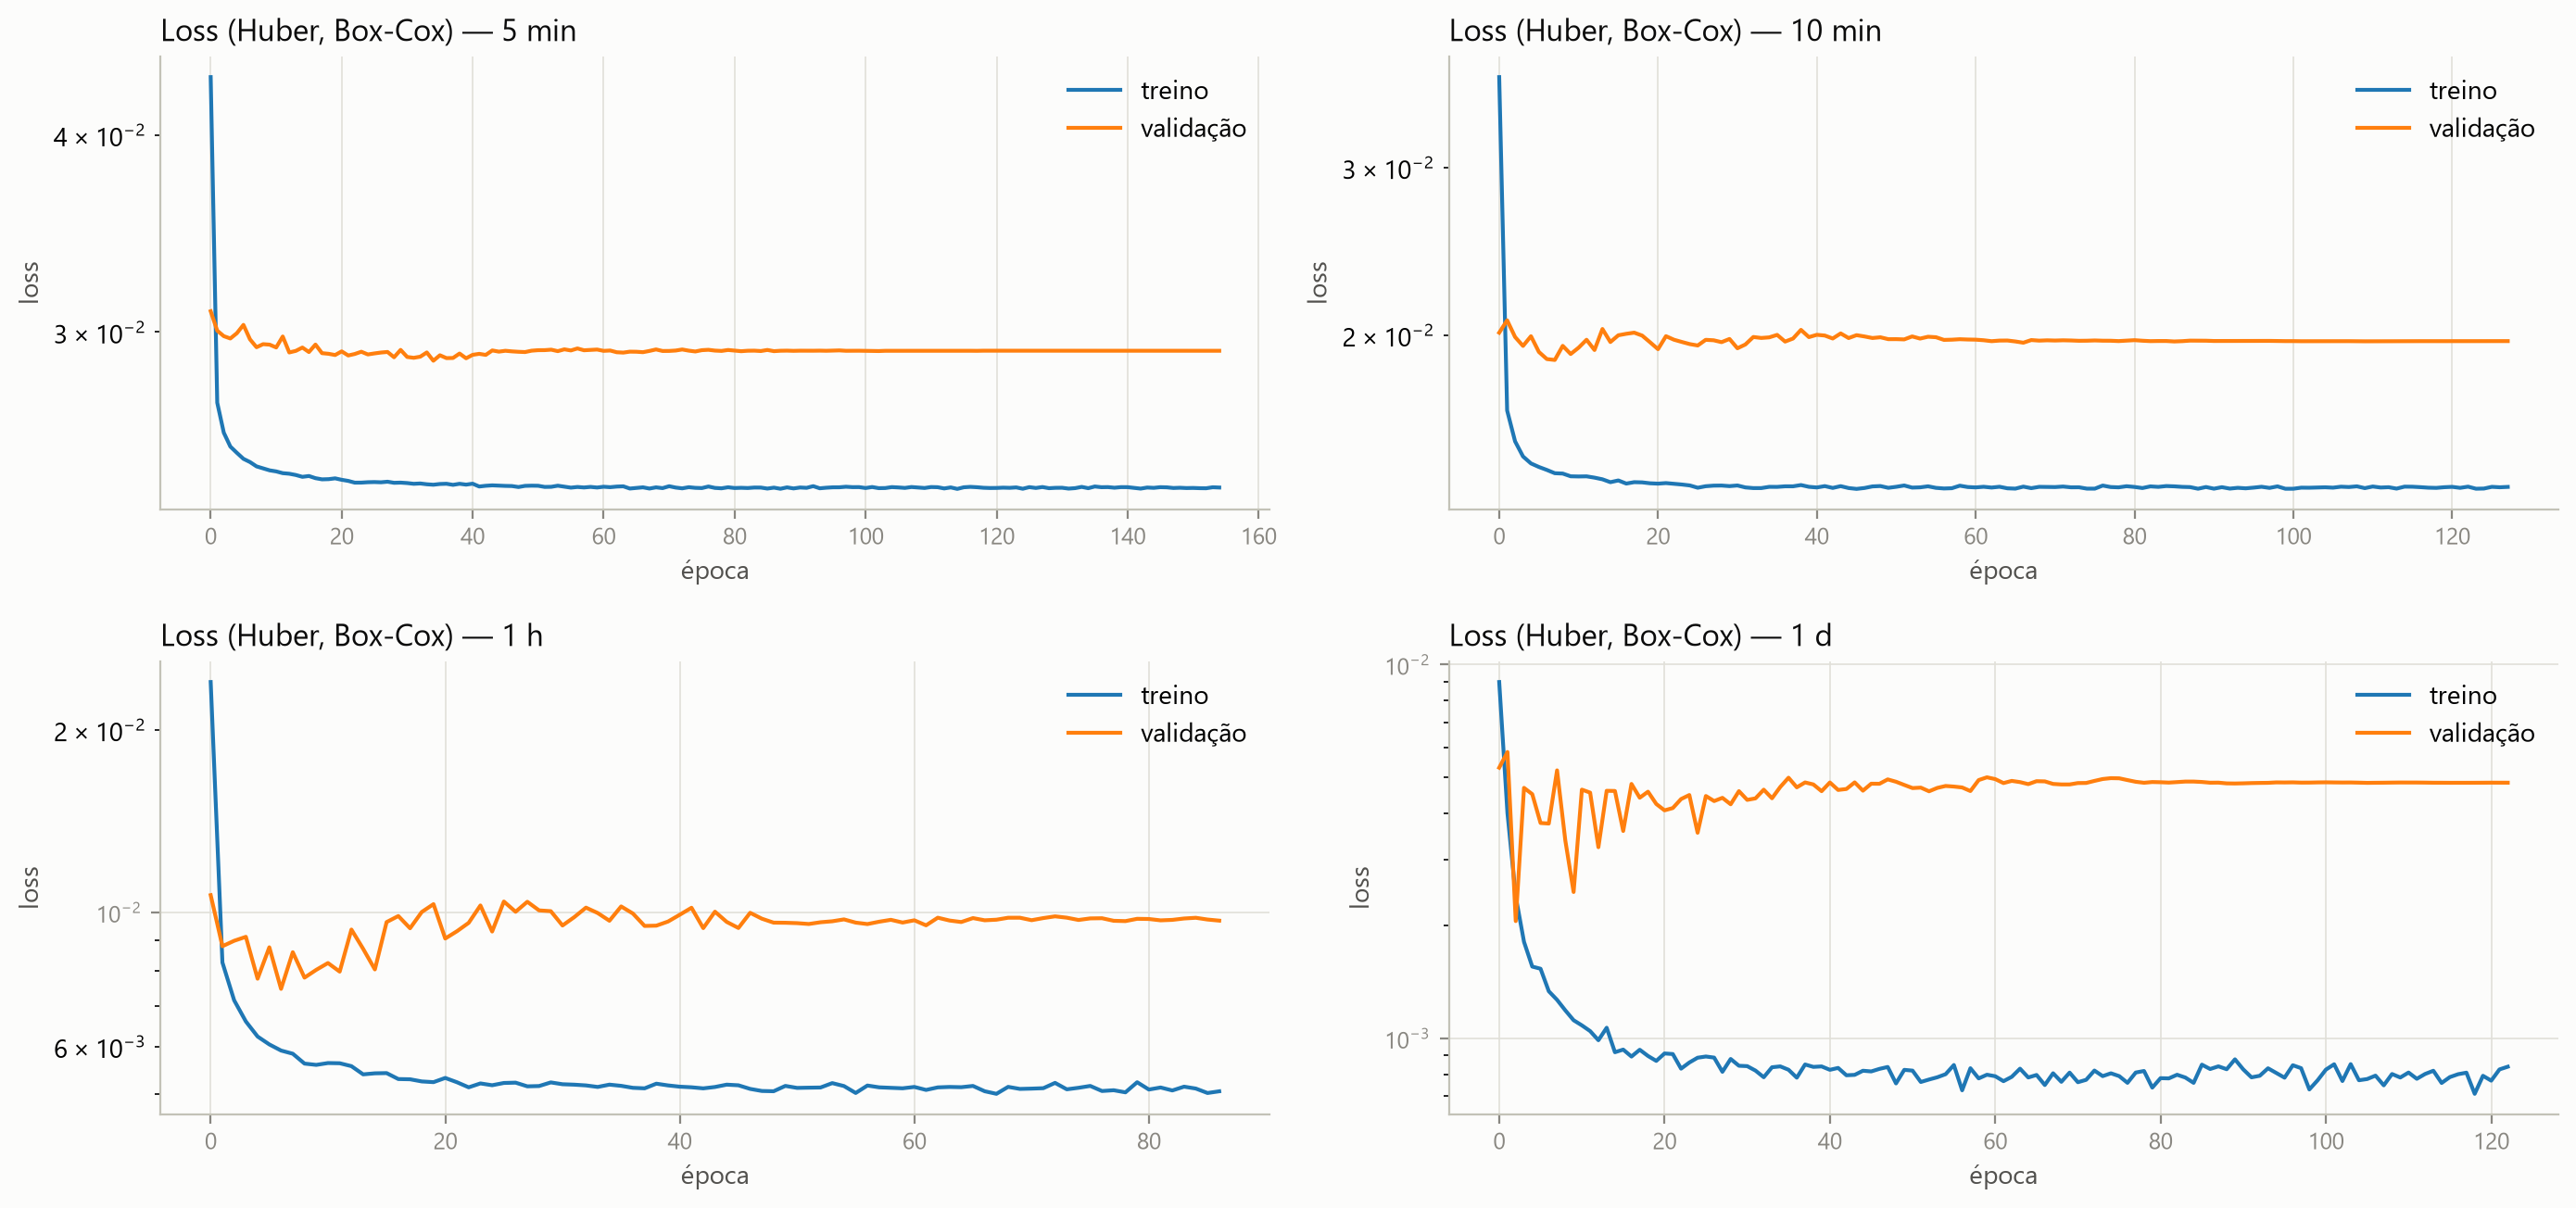
\includegraphics[width=\textwidth]{figuras/mlp_treino_granularidades.png}
  \caption{Evolução das métricas de treinamento e validação do MLP nas quatro granularidades.}
  \label{fig:mlp-treino}
  \source{Elaborado pelo autor.}
\end{figure}

\begin{figure}[H]
  \centering
  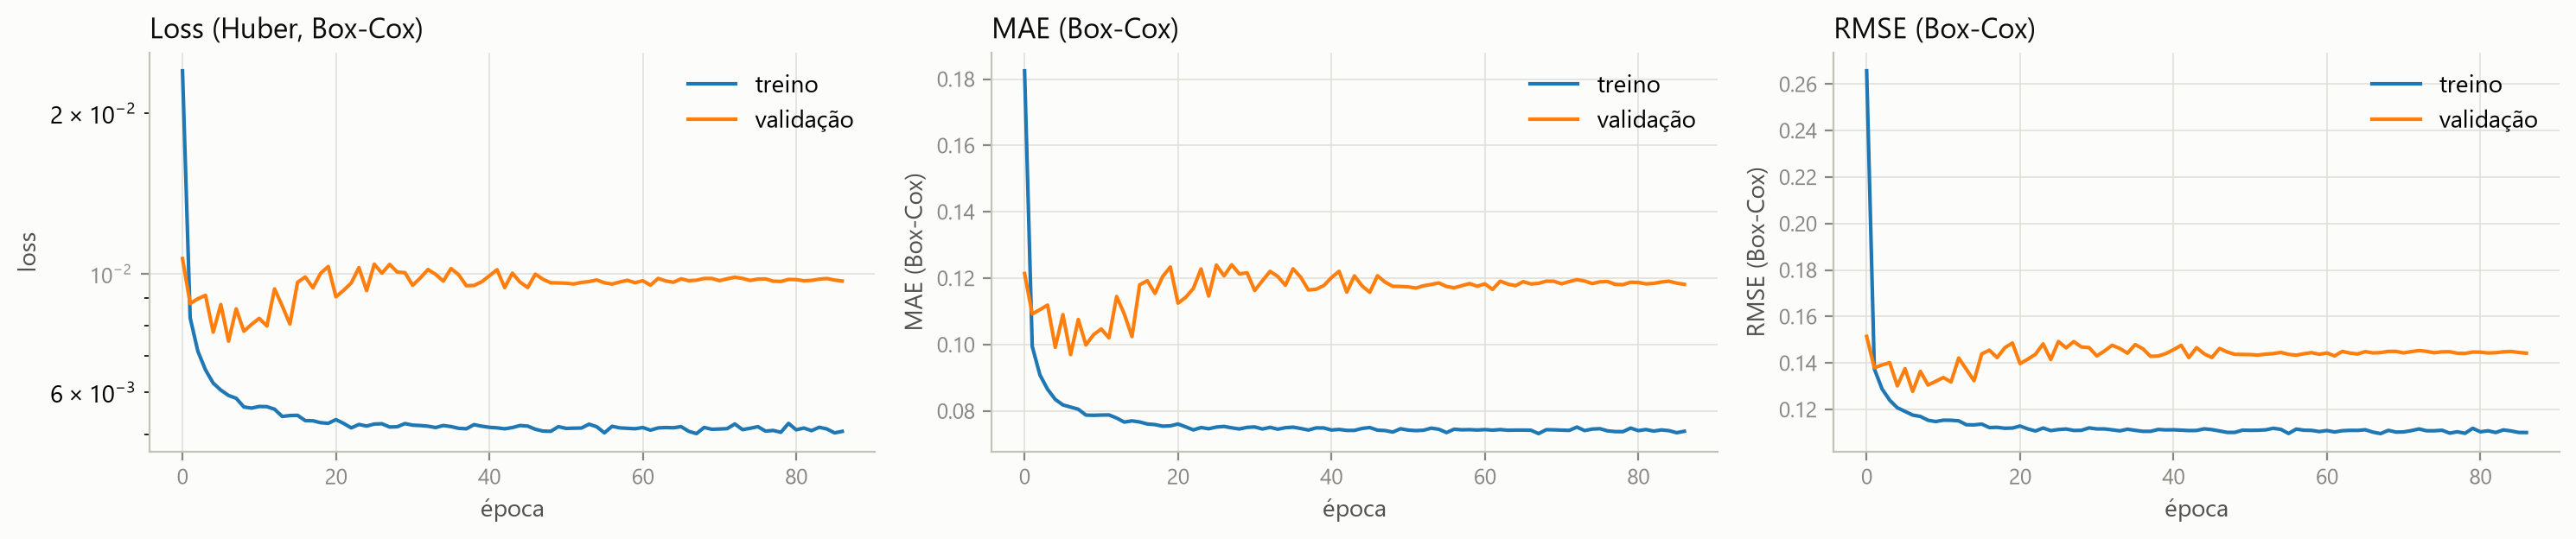
\includegraphics[width=\textwidth]{figuras/mlp_treino_1h.png}
  \caption{Curvas de perda, MAE e RMSE do treinamento do MLP na granularidade de 1~h.}
  \label{fig:mlp-treino-1h}
  \source{Elaborado pelo autor.}
\end{figure}

\section{Desempenho Offline no Teste de 2025}
\label{sec:resultados-offline}

A \cref{tab:comparativo} apresenta as métricas obtidas pelos três modelos
nos conjuntos de teste de 2025 do inversor E1. Os resultados de RF e MLP
consideram a correção de viés estimada na janela 2024H2; a regressão linear
corresponde à linha de base ajustada sem essa correção.

\begin{table}[H]
  \centering
  \caption{Métricas dos três modelos nos conjuntos de teste de 2025 do inversor E1.}
  \label{tab:comparativo}
  \resizebox{\textwidth}{!}{%
  \begin{tabular}{llrrrr}
    \toprule
    Granularidade & Modelo & MAE (kW) & RMSE (kW) & $R^2$ & Viés (kW) \\
    \midrule
    5 min  & Regressão linear & 0,1999 & 0,2775 & 0,7426 & $+0,1059$ \\
    5 min  & Random Forest    & 0,1637 & 0,2414 & 0,8052 & $+0,0130$ \\
    5 min  & MLP              & 0,1596 & 0,2398 & 0,8078 & $+0,0122$ \\
    \midrule
    10 min & Regressão linear & 0,1561 & 0,2071 & 0,8457 & $+0,1130$ \\
    10 min & Random Forest    & 0,1142 & 0,1582 & 0,9100 & $+0,0062$ \\
    10 min & MLP              & 0,1104 & 0,1552 & 0,9134 & $+0,0057$ \\
    \midrule
    1 h    & Regressão linear & 0,1168 & 0,1531 & 0,9048 & $+0,1140$ \\
    1 h    & Random Forest    & 0,0664 & 0,0835 & 0,9717 & $+0,0024$ \\
    1 h    & MLP              & 0,0543 & 0,0688 & 0,9807 & $+0,0028$ \\
    \midrule
    1 d    & Regressão linear & 0,1199 & 0,1325 & 0,5338 & $+0,1199$ \\
    1 d    & Random Forest    & 0,0396 & 0,0535 & 0,9240 & $+0,0130$ \\
    1 d    & MLP              & 0,0366 & 0,0471 & 0,9411 & $+0,0079$ \\
    \bottomrule
  \end{tabular}}
  \source{Elaborado pelo autor.}
\end{table}

O MLP apresentou o menor MAE e o maior $R^2$ nas quatro granularidades.
Em relação ao RF, a diferença de MAE foi de 0,0041~kW em 5~min,
0,0038~kW em 10~min, 0,0121~kW em 1~h e 0,0030~kW em 1~d. O viés dos dois
modelos não lineares permaneceu próximo de zero após a calibração: entre
$+0,0024$ e $+0,0130$~kW para o RF e entre $+0,0028$ e $+0,0122$~kW para o
MLP.

\begin{figure}[H]
  \centering
  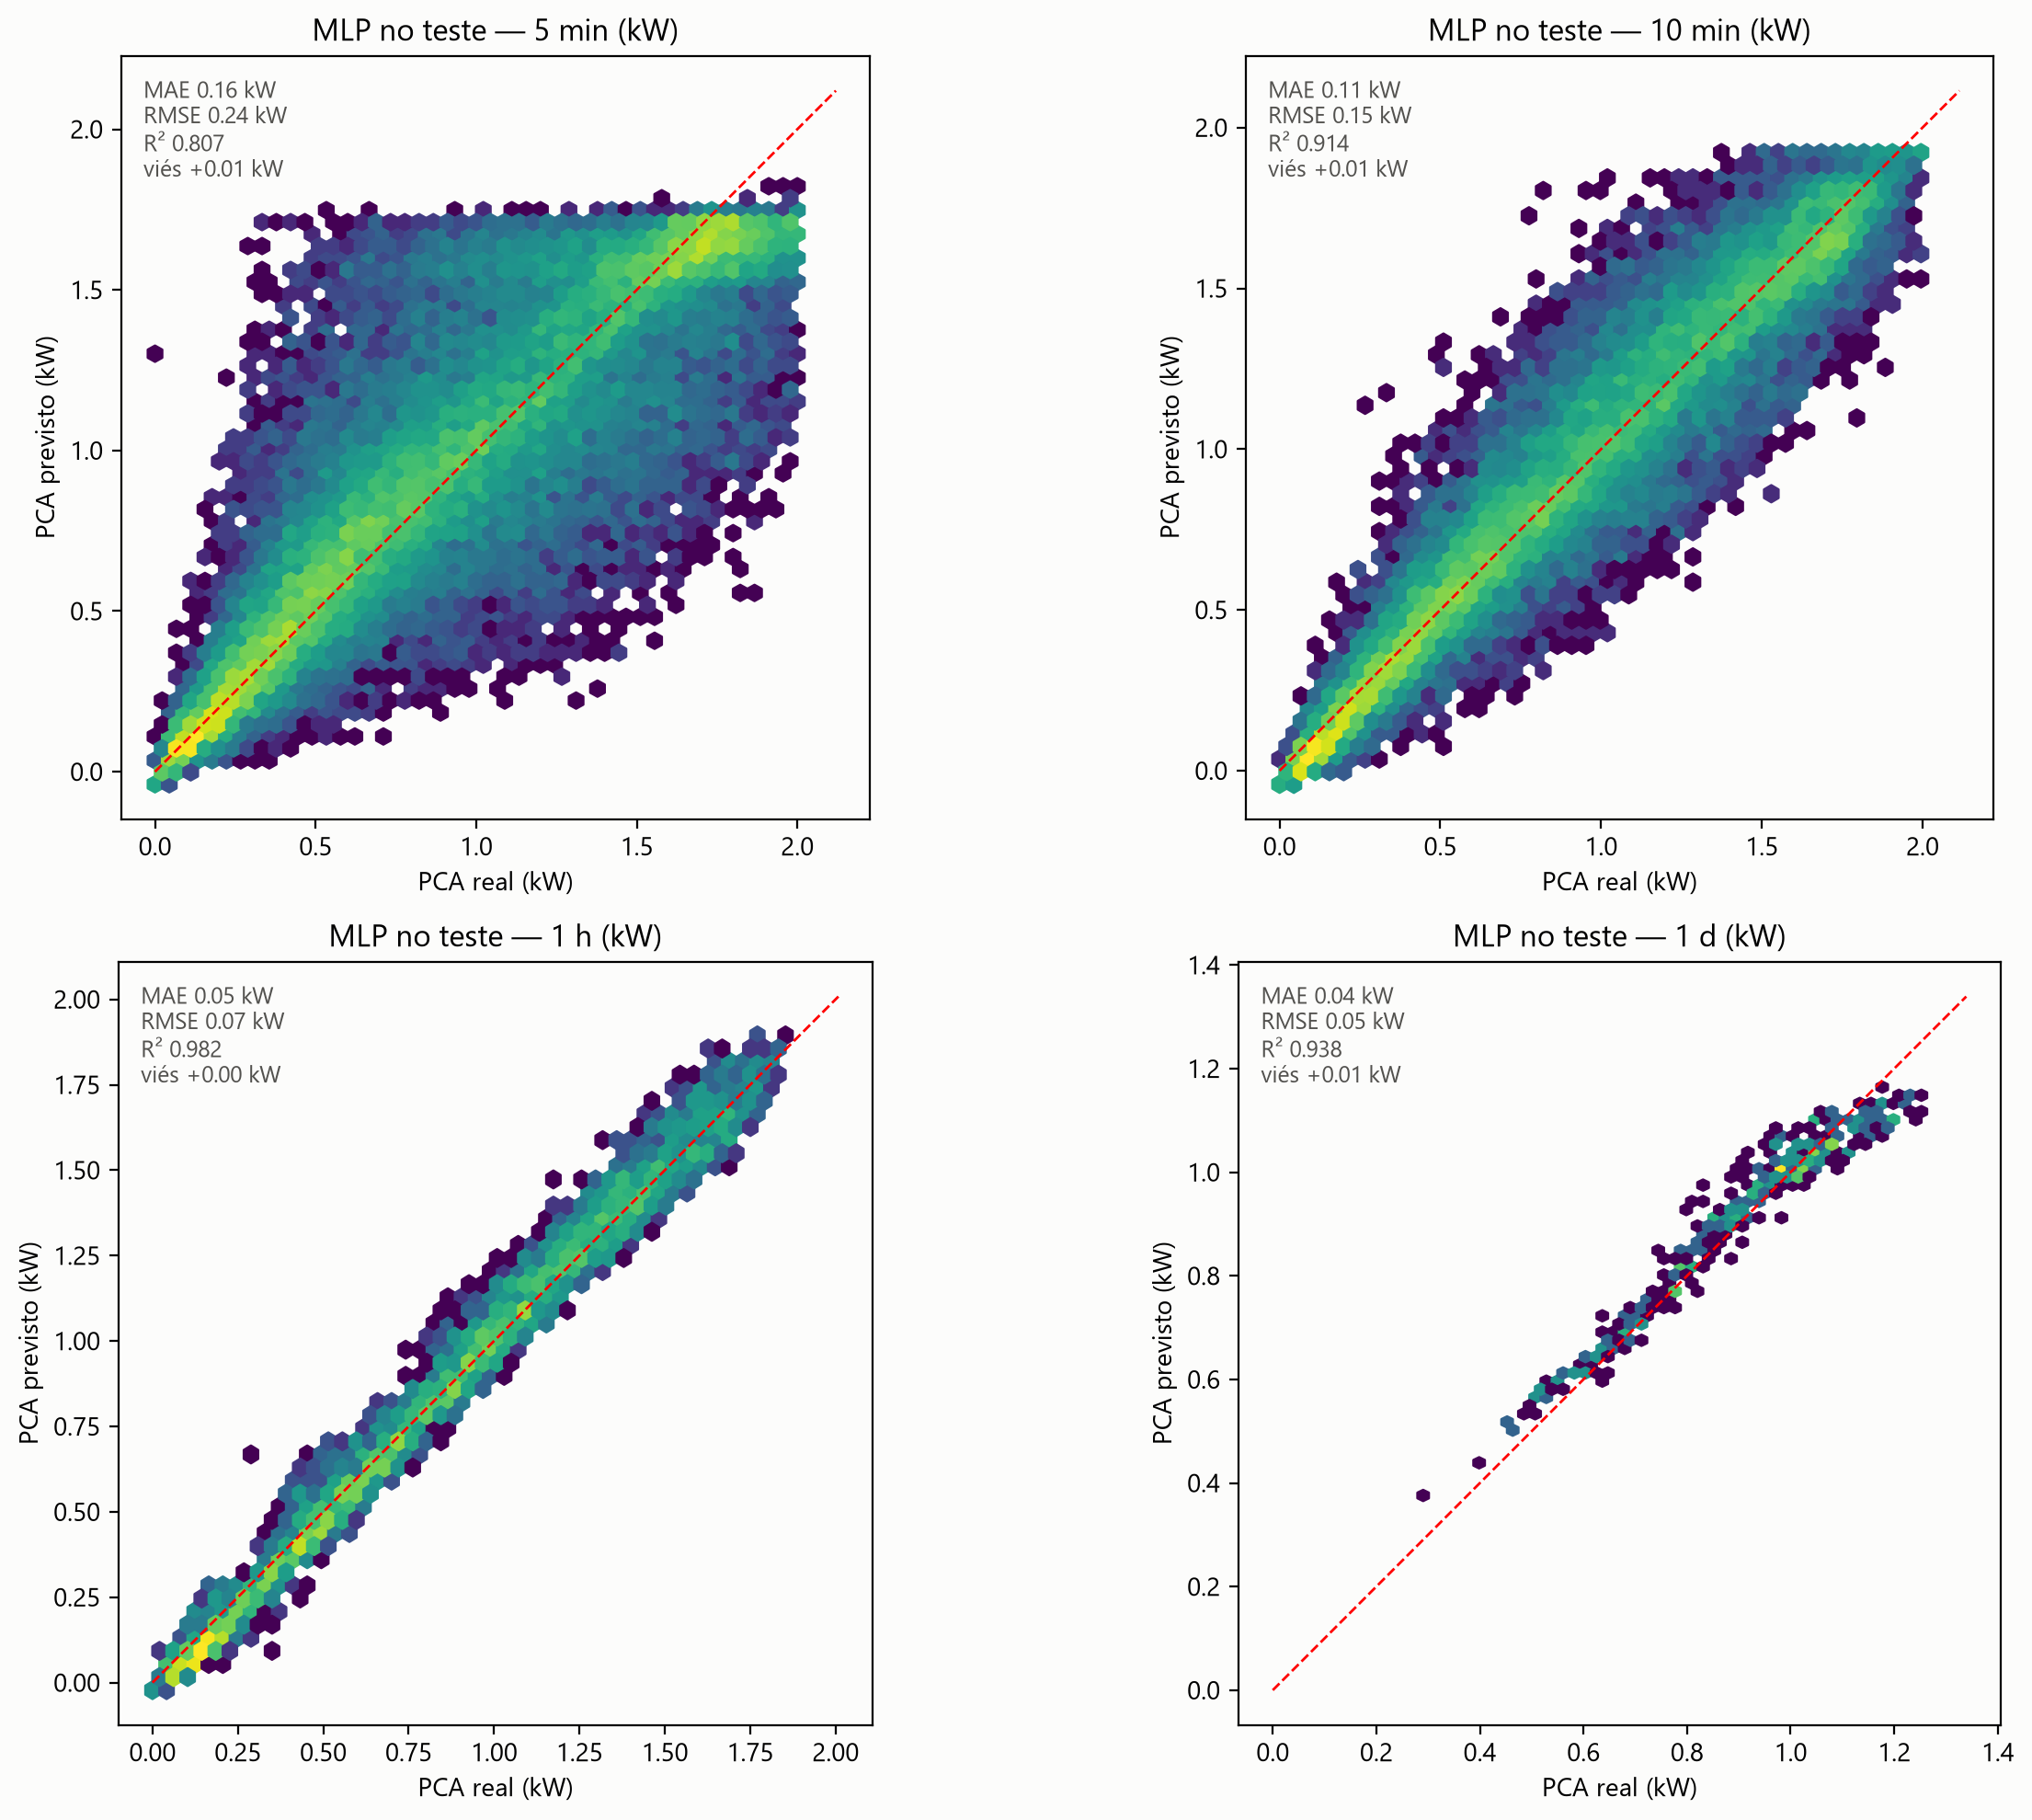
\includegraphics[width=\textwidth]{figuras/mlp_avaliacao_granularidades.png}
  \caption{Potência estimada em função da potência medida pelo MLP nos conjuntos de teste de 2025, por granularidade.}
  \label{fig:mlp-avaliacao}
  \source{Elaborado pelo autor.}
\end{figure}

\begin{figure}[H]
  \centering
  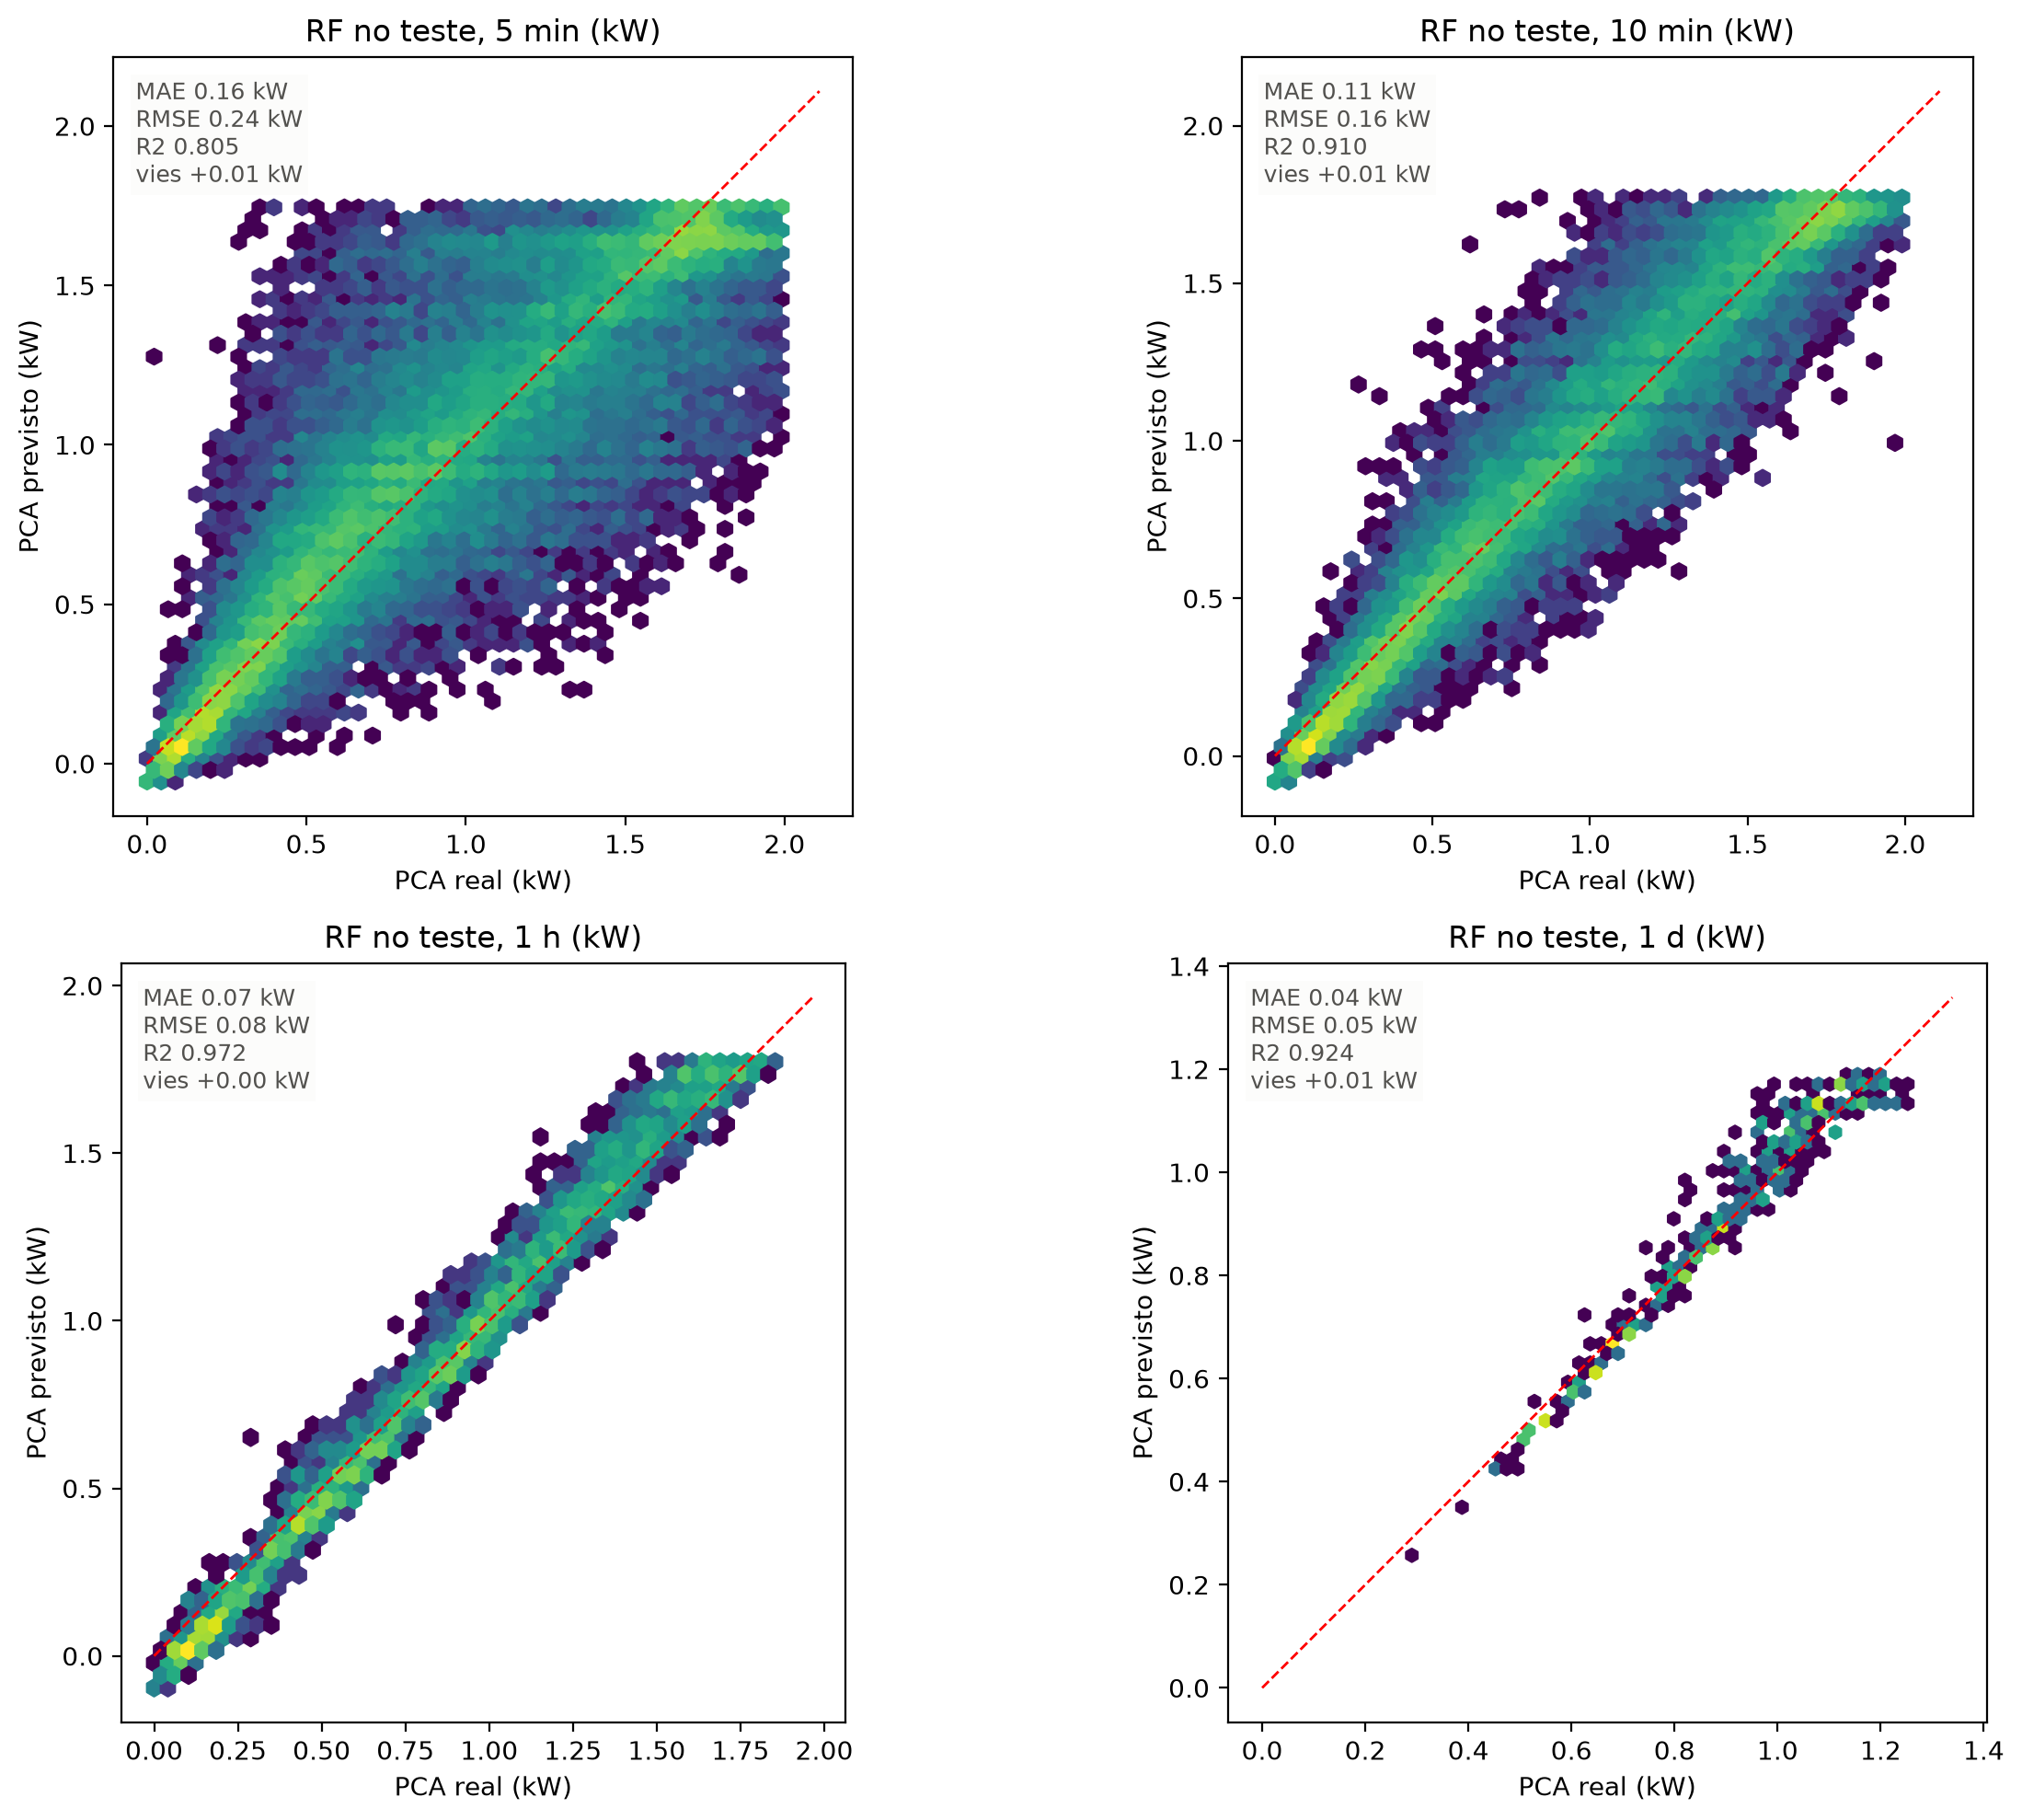
\includegraphics[width=\textwidth]{figuras/rf_avaliacao_granularidades.png}
  \caption{Potência estimada em função da potência medida pelo Random Forest nos conjuntos de teste de 2025, por granularidade.}
  \label{fig:rf-avaliacao}
  \source{Elaborado pelo autor.}
\end{figure}

O MAE dos modelos não lineares apresentou valores menores nas granularidades
mais grossas. Para o MLP, o valor passou de 0,1596~kW em 5~min para
0,0366~kW em 1~d; para o RF, passou de 0,1637~kW para 0,0396~kW. Como cada
granularidade corresponde a um alvo agregado em uma janela temporal distinta,
esses valores descrevem tarefas de estimação com resoluções diferentes.

A regressão linear apresentou métricas inferiores às dos modelos não
lineares nas quatro granularidades. A diferença mais acentuada ocorreu em
1~d: a regressão obteve $R^2=0,5338$, enquanto RF e MLP alcançaram,
respectivamente, $R^2=0,9240$ e $R^2=0,9411$.

Como referência adicional, foi avaliado um previsor constante que atribuiu
a todas as amostras a média do alvo no conjunto de treinamento. No teste de
2025, esse previsor apresentou MAE de 0,4288~kW, viés de $+0,0212$~kW e
$R^2=-0,0018$. Essa referência corresponde à previsão da média, não à
regressão linear múltipla apresentada na \cref{tab:comparativo}.

\section{Avaliação Cruzada entre Granularidades}

As \cref{tab:mlp-cruzada,tab:rf-cruzada} apresentam os valores de $R^2$ na
avaliação cruzada. Em cada matriz, as linhas correspondem à granularidade de
treinamento e as colunas à granularidade de avaliação.

\begin{table}[H]
  \centering
  \caption{$R^2$ do MLP no teste de 2025 por granularidade de treinamento (linhas) e de avaliação (colunas).}
  \label{tab:mlp-cruzada}
  \begin{tabular}{lrrrr}
    \toprule
    Treinado em & 5 min & 10 min & 1 h & 1 d \\
    \midrule
    5 min  & 0,8078 & 0,9130 & 0,9725 & 0,7671 \\
    10 min & 0,7946 & 0,9134 & 0,9788 & 0,8542 \\
    1 h    & 0,7844 & 0,9100 & 0,9807 & 0,8868 \\
    1 d    & 0,6959 & 0,7886 & 0,8682 & 0,9411 \\
    \bottomrule
  \end{tabular}
  \source{Elaborado pelo autor.}
\end{table}

\begin{table}[H]
  \centering
  \caption{$R^2$ do Random Forest no teste de 2025 por granularidade de treinamento (linhas) e de avaliação (colunas).}
  \label{tab:rf-cruzada}
  \begin{tabular}{lrrrr}
    \toprule
    Treinado em & 5 min & 10 min & 1 h & 1 d \\
    \midrule
    5 min  & 0,8052 & 0,9083 & 0,9649 & 0,6982 \\
    10 min & 0,7940 & 0,9100 & 0,9731 & 0,8046 \\
    1 h    & 0,7774 & 0,9029 & 0,9717 & 0,8609 \\
    1 d    & 0,6402 & 0,7280 & 0,8269 & 0,9240 \\
    \bottomrule
  \end{tabular}
  \source{Elaborado pelo autor.}
\end{table}

\begin{figure}[H]
  \centering
  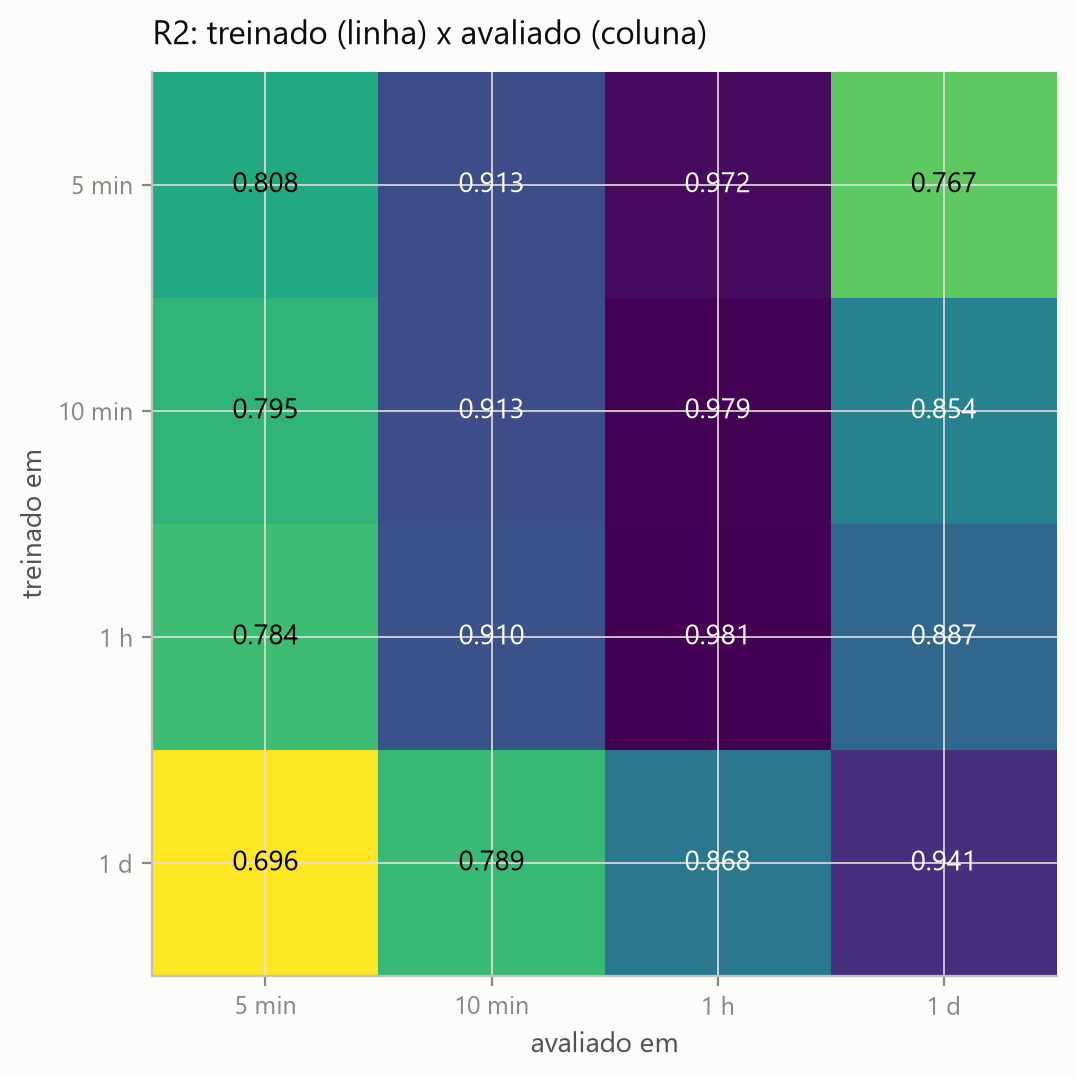
\includegraphics[width=0.78\textwidth]{figuras/mlp_cruzada.png}
  \caption{Matriz de avaliação cruzada do MLP, expressa pelo coeficiente de determinação ($R^2$).}
  \label{fig:mlp-cruzada}
  \source{Elaborado pelo autor.}
\end{figure}

\begin{figure}[H]
  \centering
  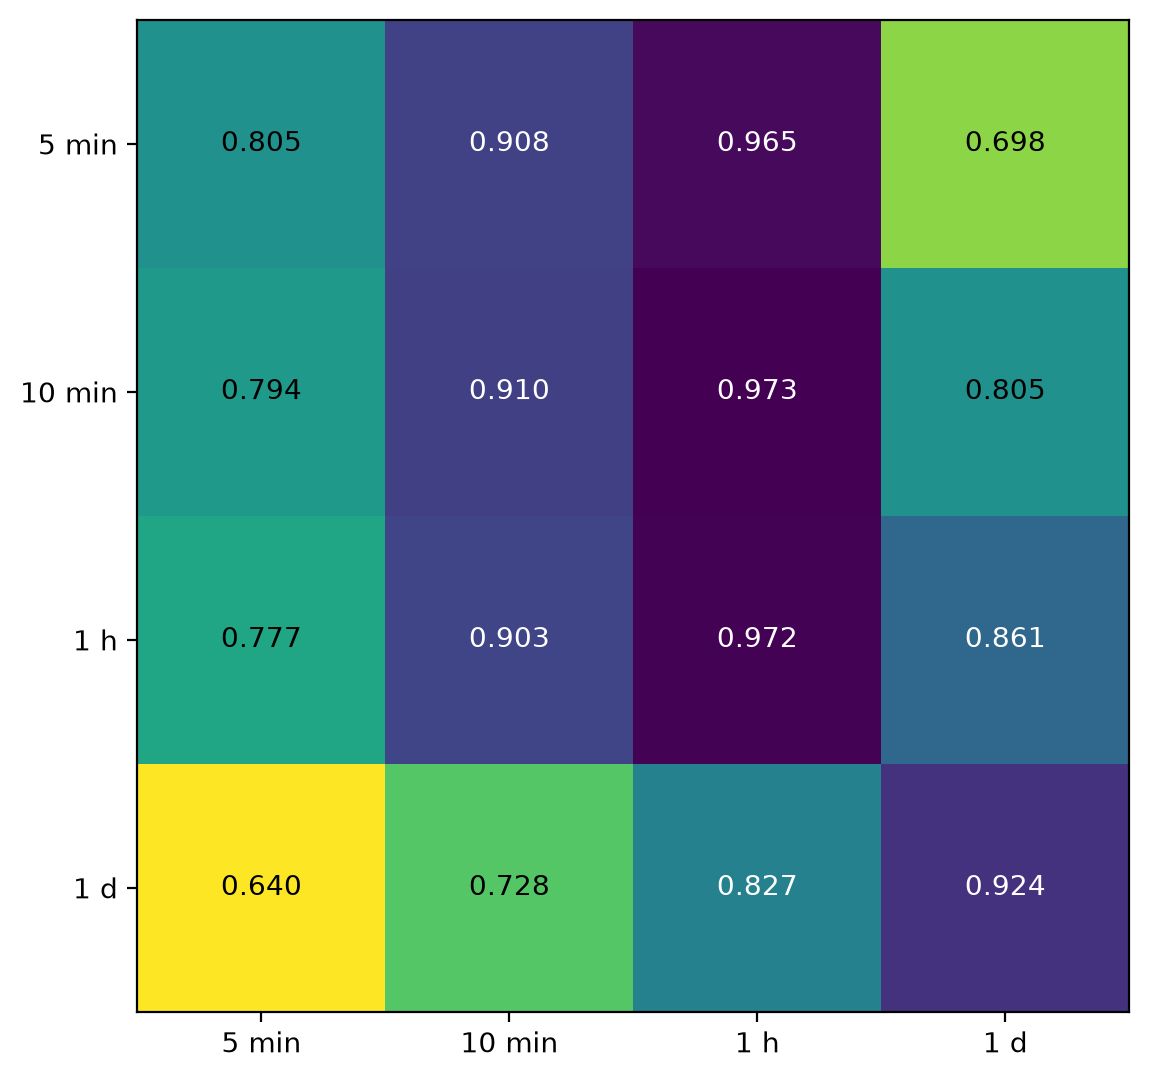
\includegraphics[width=0.78\textwidth]{figuras/rf_cruzada.png}
  \caption{Matriz de avaliação cruzada do Random Forest, expressa pelo coeficiente de determinação ($R^2$).}
  \label{fig:rf-cruzada}
  \source{Elaborado pelo autor.}
\end{figure}

Os dois modelos mantiveram valores positivos de $R^2$ em todas as
combinações avaliadas. Quando treinado em 1~h e avaliado em 5~min, o MLP
obteve $R^2=0,7844$ e o RF, $R^2=0,7774$. Para o treinamento em 10~min e
a avaliação em 5~min, os valores foram 0,7946 e 0,7940, respectivamente.

Nas avaliações em 1~h, os modelos treinados em granularidades mais finas
apresentaram $R^2$ acima de 0,96. Por outro lado, a maior redução ocorreu
quando os modelos treinados em 1~d foram avaliados em 5~min: o MLP obteve
$R^2=0,6959$ e o RF, $R^2=0,6402$. Na avaliação desses mesmos modelos em
1~h, os valores foram 0,8682 e 0,8269, respectivamente. O MLP apresentou
$R^2$ superior ao RF em todas as células das matrizes.

\section{Avaliação das Variantes de Quantização do MLP}

A \cref{tab:quantizacao-mlp} apresenta o tamanho e as métricas obtidas para
as variantes do MLP de 1~h. A variante \texttt{int8} utilizada no firmware
apresentou MAE de 0,0555~kW, diferença de 0,0005~kW em relação à variante
\texttt{float32}. O tamanho do modelo foi reduzido de 44,86~KB para
19,27~KB, redução de aproximadamente 57\%.

\begin{table}[H]
  \centering
  \caption{Tamanho e desempenho das variantes de quantização do MLP de 1~h no teste de 2025.}
  \label{tab:quantizacao-mlp}
  \resizebox{\textwidth}{!}{%
  \begin{tabular}{lrrrrr}
    \toprule
    Variante & Tamanho (KB) & MAE (kW) & RMSE (kW) & $R^2$ & Viés (kW) \\
    \midrule
    \texttt{float32} & 44,86 & 0,0550 & 0,0697 & 0,9803 & $+0,0035$ \\
    \texttt{float16} & 24,86 & 0,0550 & 0,0697 & 0,9803 & $+0,0036$ \\
    Dinâmica & 16,08 & 0,0552 & 0,0700 & 0,9802 & $+0,0041$ \\
    \texttt{int8} (entrada e saída \texttt{int8}) & 19,27 & 0,0555 & 0,0707 & 0,9798 & $+0,0055$ \\
    \texttt{int8} (entrada e saída \texttt{float}) & 19,60 & 0,0555 & 0,0707 & 0,9798 & $+0,0055$ \\
    \bottomrule
  \end{tabular}}
  \source{Elaborado pelo autor.}
\end{table}

A quantização dinâmica produziu o menor arquivo, com 16,08~KB, mas essa
variante não foi ensaiada na placa. O mesmo ocorreu com as variantes
\texttt{float16} e \texttt{int8} com entrada e saída em ponto flutuante.
As diferenças após o recálculo da correção de calibração na janela 2024H2
ficaram na terceira ou quarta casa decimal das métricas.

\section{Ensaio Embarcado}
\label{sec:ensaio-embarcado}

\subsection{Tempo de execução observado}

Nos ensaios registrados, o processamento de cada lote de até 64 amostras
levou de 75 a 96~ms. Para o RF, os tempos observados ficaram entre 90 e
96~ms por lote; para o MLP com TensorFlow Lite, entre 75 e 81~ms. Esses
intervalos correspondem a aproximadamente 670 a 850 amostras por segundo.
Um conjunto de 4\,042 linhas foi processado em aproximadamente 6 a 8~s.
A taxa observada decorreu da execução em lotes, sem espera pelo período
nominal de operação dos modelos.

Os logs finais de 12 de novembro de 2026 não registraram falhas. Em logs
anteriores, foram registradas tentativas de retomada por meio de
\texttt{RESUME} e reenvio de lotes, sem perda ou duplicação de linhas no
resultado consolidado.

\subsection{Random Forest de 1 h com lacunas artificiais no inversor E1}

No ensaio embarcado do RF de 1~h no inversor E1, foram transmitidas as
4\,042 linhas do conjunto de teste de 2025. Destas, 775 correspondiam a
amostras localizadas em lacunas artificiais. Fora das lacunas, as métricas
obtidas na placa ficaram próximas às da avaliação offline, conforme a
\cref{tab:rf-placa-offline}.

\begin{table}[H]
  \centering
  \caption{Métricas do Random Forest de 1~h fora das lacunas no ensaio embarcado e na avaliação offline.}
  \label{tab:rf-placa-offline}
  \begin{tabular}{lrr}
    \toprule
    Métrica & Fora das lacunas & Offline (referência) \\
    \midrule
    MAE (kW) & 0,066 & 0,0664 \\
    RMSE (kW) & 0,083 & 0,0835 \\
    $R^2$ & 0,972 & 0,9717 \\
    Viés (kW) & $+0,003$ & $+0,0024$ \\
    \bottomrule
  \end{tabular}
  \source{Elaborado pelo autor.}
\end{table}

Dentro das lacunas, o MAE do \textit{soft-sensor} foi de 0,065~kW. Para
o mesmo conjunto de amostras, a interpolação linear apresentou MAE de
0,312~kW e a persistência do último valor observado, 0,376~kW. A
\cref{tab:ensaio-gaps} apresenta os erros por duração dos blocos. Nos blocos
contínuos, o MAE do \textit{soft-sensor} variou de 0,037 a 0,071~kW. Para a
interpolação linear, os valores variaram de 0,220 a 0,505~kW; para a
persistência, de 0,269 a 0,491~kW. Nas falhas esporádicas, o MAE foi de
0,063~kW para o \textit{soft-sensor}, 0,150~kW para a interpolação e
0,276~kW para a persistência.

\begin{table}[H]
  \centering
  \caption{Erro dentro das lacunas por duração do bloco no ensaio RF-1H no inversor E1.}
  \label{tab:ensaio-gaps}
  \resizebox{\textwidth}{!}{%
  \begin{tabular}{lrrrr}
    \toprule
    Duração do bloco & Amostras & \textit{Soft-sensor} (kW) & Interpolação (kW) & Persistência (kW) \\
    \midrule
    1 h & 4 & 0,037 & 0,220 & 0,269 \\
    6 h & 24 & 0,069 & 0,374 & 0,438 \\
    24 h & 96 & 0,071 & 0,505 & 0,491 \\
    3 dias & 288 & 0,066 & 0,447 & 0,459 \\
    Esporádica & 363 & 0,063 & 0,150 & 0,276 \\
    Total dentro das lacunas & 775 & 0,065 & 0,312 & 0,376 \\
    \bottomrule
  \end{tabular}}
  \source{Elaborado pelo autor.}
\end{table}

A \cref{fig:ensaio-gap} apresenta a série no maior bloco contínuo, com
72~h, e a \cref{fig:ensaio-gaps-duracao} reúne os resultados por duração
das lacunas artificiais.

\begin{figure}[H]
  \centering
  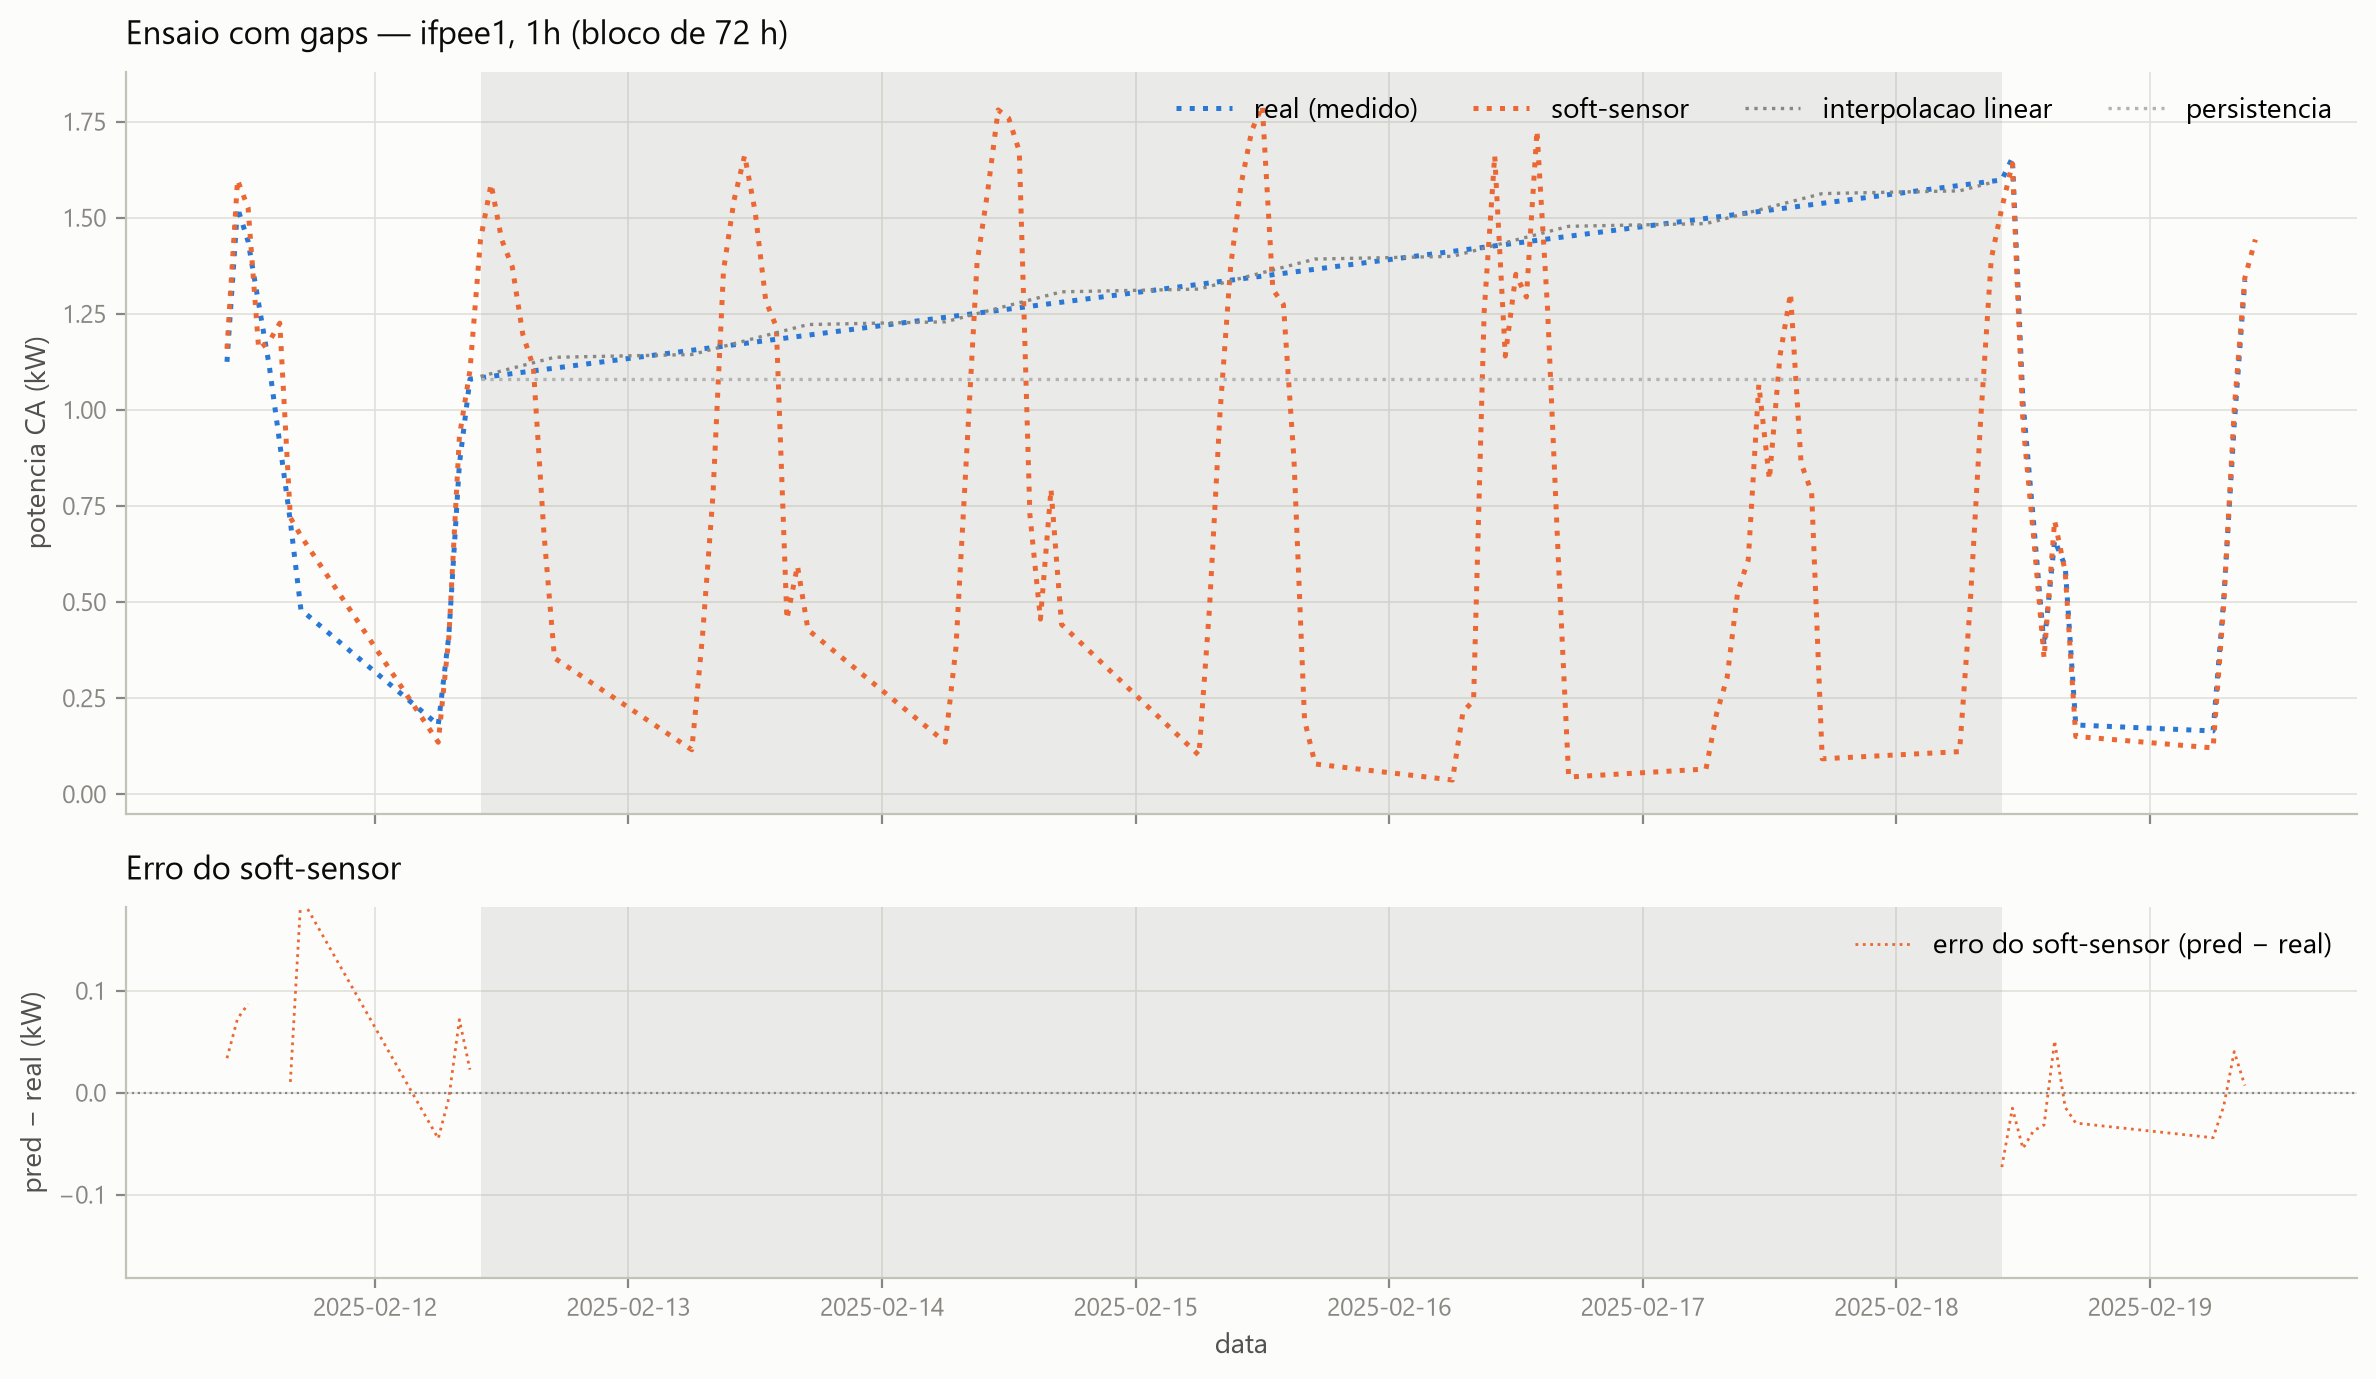
\includegraphics[width=\textwidth]{figuras/ensaio_gap_ifpee1.png}
  \caption{Série medida e estimativas no ensaio embarcado com uma lacuna artificial de 72~h no inversor E1.}
  \label{fig:ensaio-gap}
  \source{Elaborado pelo autor.}
\end{figure}

\begin{figure}[H]
  \centering
  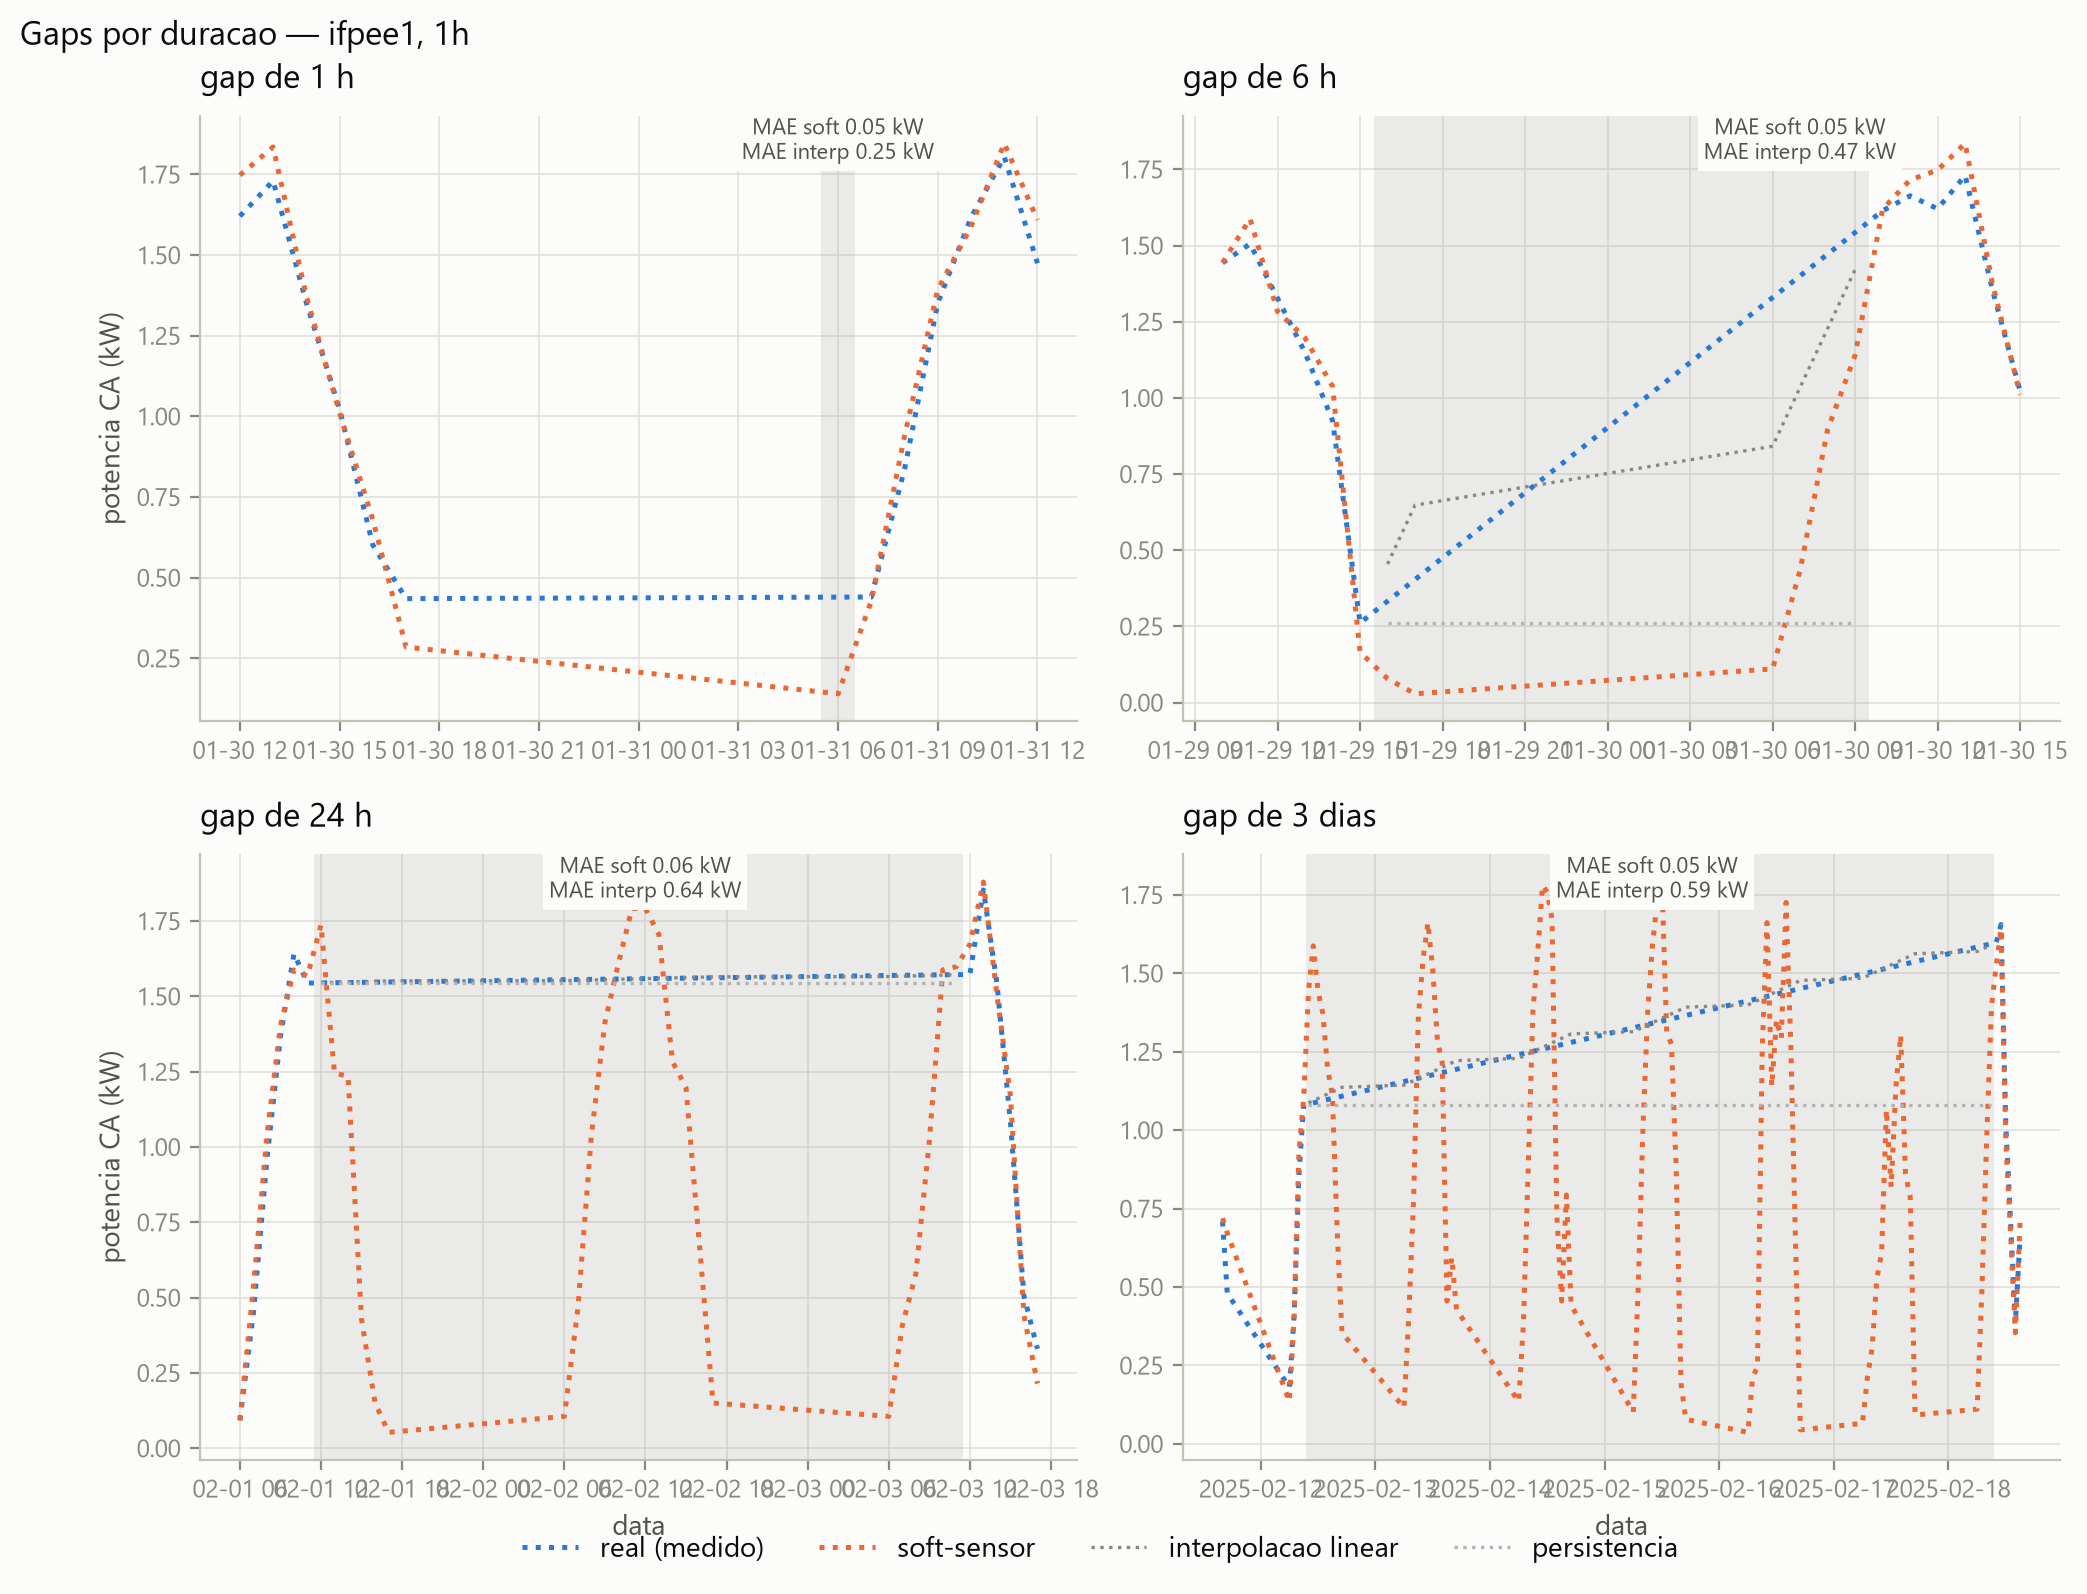
\includegraphics[width=0.92\textwidth]{figuras/ensaio_gaps_duracao_ifpee1.png}
  \caption{Resultados do ensaio embarcado do Random Forest por duração das lacunas artificiais no inversor E1.}
  \label{fig:ensaio-gaps-duracao}
  \source{Elaborado pelo autor.}
\end{figure}

\subsection{MLP de 1 h quantizado em \texttt{int8}}

No ensaio embarcado do MLP de 1~h quantizado em \texttt{int8}, o painel do
servidor registrou 4\,039 observações válidas a partir das 4\,042 linhas
transmitidas. As métricas reportadas foram MAE de 0,05~kW, RMSE de
0,07~kW, $R^2=0,981$, viés de $+0,00$~kW, MAPE de 11,9\% e percentil 90 do
erro absoluto de 0,11~kW, conforme a \cref{tab:mlp-placa}.

\begin{table}[H]
  \centering
  \caption{Métricas reportadas pelo painel no ensaio embarcado do MLP de 1~h quantizado em \texttt{int8}.}
  \label{tab:mlp-placa}
  \begin{tabular}{lr}
    \toprule
    Métrica & Valor \\
    \midrule
    MAE & 0,05~kW \\
    RMSE & 0,07~kW \\
    $R^2$ & 0,981 \\
    Viés & $+0,00$~kW \\
    MAPE & 11,9\% \\
    P90 do erro absoluto & 0,11~kW \\
    \bottomrule
  \end{tabular}
  \source{Elaborado pelo autor a partir do painel do ensaio.}
\end{table}

Na análise mensal, o MAE variou entre 0,04 e 0,11~kW, enquanto o $R^2$
ficou entre 0,939 e 0,987. Dezembro apresentou o maior MAE (0,11~kW) e o
menor $R^2$ informado (0,939). Julho apresentou o menor MAE (0,04~kW), com
$R^2=0,985$. No agregado, os valores reportados pelo painel ficaram próximos
aos da avaliação offline do MLP de 1~h, que apresentou MAE de 0,0543~kW e
$R^2=0,9807$.

\subsection{Custo de memória e tamanho dos artefatos}

A \cref{tab:custo-embarcado} reúne as medidas de tamanho dos modelos e dos
artefatos compilados. Para o RF, a medida de flash corresponde ao objeto
Xtensa da biblioteca C compilado com otimização \texttt{-O2}; não representa
o firmware completo. A compilação final do firmware RF, com a otimização
\texttt{-Os}, não estava disponível no momento da medição. Para o MLP,
foram registrados o tamanho do modelo, a arena de tensores e as seções do
firmware compilado.

\begin{table}[H]
  \centering
  \caption{Tamanho dos modelos e consumo de memória medido nos artefatos embarcados.}
  \label{tab:custo-embarcado}
  \resizebox{\textwidth}{!}{%
  \begin{tabular}{p{0.73\textwidth}r}
    \toprule
    Item & Medida \\
    \midrule
    Biblioteca C do RF de 1~h (objeto Xtensa, \texttt{-O2}) & 486\,267 bytes (474,9~KB) \\
    RAM de dados da biblioteca C do RF de 1~h & 0 bytes \\
    Modelo MLP \texttt{int8} de 1~h (arquivo \texttt{.tflite}) & 19\,736 bytes (19,3~KB) \\
    Arena de tensores do TensorFlow Lite Micro & 8\,192 bytes \\
    Firmware \texttt{mlp-tflite}, seção \texttt{text} & 241\,249 bytes \\
    Firmware \texttt{mlp-tflite}, seção \texttt{data} & 109\,844 bytes \\
    Flash aproximada (\texttt{text} + \texttt{data}) & 351\,093 bytes \\
    Firmware \texttt{mlp-tflite}, seção \texttt{bss} & 254\,505 bytes \\
    Arquivo \texttt{firmware.bin} do \texttt{mlp-tflite} & 351\,200 bytes \\
    \bottomrule
  \end{tabular}}
  \source{Elaborado pelo autor.}
\end{table}

A biblioteca do RF foi emitida como código \textit{inline}, sem tabela de
parâmetros alocada em RAM, mas ocupou 474,9~KB no objeto compilado. No MLP,
o arquivo do modelo quantizado ocupou 19,3~KB e a arena do TensorFlow Lite
Micro utilizou 8\,192 bytes. O firmware completo do MLP apresentou
aproximadamente 351~KB nas seções \texttt{text} e \texttt{data}, além de
254,5~KB na seção \texttt{bss}. Como as medidas do RF e do MLP correspondem
a artefatos de escopos de compilação diferentes, a comparação direta dos
valores de flash deve ser feita com essa ressalva.

\section{Síntese dos Resultados e Escopo Experimental}

Nos testes offline de E1, o MLP apresentou o menor MAE e o maior $R^2$ entre
os modelos comparados nas quatro granularidades, com vantagem pequena sobre
o RF e resultados superiores aos da regressão linear múltipla. Na avaliação
cruzada, os dois modelos não lineares mantiveram valores positivos de $R^2$
nas combinações examinadas. A maior redução ocorreu na transferência dos
modelos treinados em 1~d para dados de 5~min. A quantização \texttt{int8} do
MLP de 1~h reduziu o tamanho do modelo em aproximadamente 57\% em relação à
variante \texttt{float32}, com diferença de 0,0005~kW no MAE reportado.

Nos ensaios embarcados realizados em E1, as métricas do RF fora das lacunas
ficaram próximas às da avaliação offline. Dentro das lacunas artificiais, o
MAE do \textit{soft-sensor} foi inferior aos das referências de interpolação
linear e persistência. O ensaio separado do MLP \texttt{int8} também
apresentou métricas próximas às obtidas na avaliação offline. As execuções
foram realizadas em hardware real com reprodução de dados históricos pelo
host; não constituíram operação de campo com aquisição direta dos sensores.

Entre as oito combinações de modelo e granularidade previstas na matriz
experimental, os resultados disponíveis neste capítulo abrangem o ensaio de
lacunas do RF de 1~h em E1 e um ensaio embarcado separado do MLP de 1~h
quantizado em \texttt{int8}, também em E1. As demais combinações e os ensaios
embarcados nos inversores E2 e E3 permaneciam pendentes no conjunto de
resultados utilizado. Embora as séries de teste de E2 e E3 tenham sido
preparadas, não são apresentados neste capítulo valores de avaliação
offline desses inversores. Assim, os resultados disponíveis ainda não
permitem comparar todas as combinações previstas nem avaliar a transferência
entre inversores em hardware.

Os resultados do MLP apresentados neste capítulo referem-se ao caminho local
\texttt{mlp-tflite}. O caminho \texttt{mlp-ei}, baseado em uma versão anterior
do impulso do Edge Impulse, não foi incluído nas comparações porque utiliza
outra ordem de eixos e outro escalonador, não correspondendo ao modelo local
atualmente utilizado.

% PENDÊNCIA DE CONSISTÊNCIA: o painel do ensaio MLP informa 4.039 observações
% válidas em 4.042 linhas transmitidas. A metodologia revisada determina que
% os zeros válidos sejam incluídos em MAE, RMSE, R^2 e viés, sendo excluídos
% apenas do MAPE. Conferir a rotina do painel e recalcular as métricas, se
% necessário, antes da versão final.
